\documentclass
[]
{thesis}

\usepackage{graphicx}
\usepackage{amsmath}
\usepackage{lipsum} 
\usepackage{hyperref}  
\usepackage{bookmark}
\usepackage{xspace}

%% set up aliases
\newcommand{\GeVc}{\ensuremath{{\,\text{Ge\hspace{-.08em}V\hspace{-0.16em}/\hspace{-0.08em}}c}}\xspace}
\newcommand{\GeVcc}{\ensuremath{{\,\text{Ge\hspace{-.08em}V\hspace{-0.16em}/\hspace{-0.08em}}c^\text{2}}}\xspace}
\newcommand{\MeVcc}{\ensuremath{{\,\text{Me\hspace{-.08em}V\hspace{-0.16em}/\hspace{-0.08em}}c^\text{2}}}\xspace}
\newcommand{\GeV}{\ensuremath{{\,\text{Ge\hspace{-.08em}V\hspace{-0.16em}}}\xspace}}

\title{Title Filler}
\titleCaps{TITLE FILLER}
\author{John Lawrence}
%\holding{}
%\seeking{}
%\degree{}
\date{May 2018}

% Administration
%\graduateDean{}
\department{Department of Physics}
%\departmentChair{}

% Supervisor (adviser / mentor)
\supervisor{Kenichi Hatakeyama}
\supervisorTitle{Director}

% Honors Program Director
\honorsProgramDirector{Elizabeth Corey}

% Abstract
\abstract{Yet to be filled in.}


\begin{document}
\pdfbookmark[-1]{CONTENT}{bookmark:Content}
	
\chapter{Basic Particle Physics and CERN}
\label{chap:intro}
Ever since ancient Greece, people have been trying to discover what makes up everything. Back then they said that everything was comprised of four elements: earth, fire, water, and air. Although modern scientists use more than four elements, they are still trying to categorize the most fundamental element that makes up everything. Democritus, an ancient Greek scientist, proposed that everything if divided enough times could be broken down into atoms at their most fundamental level. While some people named something the atom that was not the most fundamental substance, scientists today are still pursuing the "atom" theorized by Democritus, the most fundamental substance. 

In the 19th century John Dalton believed he found the most fundamental particle and named it the atom, but as time passed, there was strong evidence that even atoms had internal components and structure. This was proven when J.~J.~Thompson in the late 19th century found the electron, which proved to be a component of the atom. The electron was not only the first fundamental particle discovered, but also the beginning of particle physics as a field of study. While it was an insightful discovery that led to many inventions, there were still many unknowns about the atom. About a decade after Thompson, Robert Millikan made fine measurements of the charge and mass of the electron, but this raised even more questions about the atom. It was not until Ernest Rutherford in the early 20th century showed that the atom is mostly empty space with a very dense core called the nucleus which has an opposite charge to that of the electron. He did this by shooting alpha particles, made up of two protons and two neutrons, at gold foil and observing their scattering angle. In this experiment most of the alpha particles passed through unperturbed while a handful were majorly deflected. From this observation, Rutherford concluded that most of the atom is empty space while having a highly dense core called the nucleus. 

These discoveries showed that there were more things to explore past the atom, and in parallel there were equally important theories being developed. Quantum mechanics is essential to the study of sub-atomic particles as they no longer behave according to classical mechanics. During this development Max Planck was doing his work on the quantization of energy. This set the groundwork for quantum mechanics and also served as a basis to Einstein's work. Einstein formulated the important concept of light as a particle called the photon. Previously, light had been described as a wave but Einstein showed that light had many particle like properties and momentum. This theory and the more traditional view of light as a wave, were combined leading to the wave particle duality of light. Eventually Louis De Brogile extended this duality to all particles theorizing that all particles including electrons and other sub-atomic particles could be described using waves or particles.

Einstein's theory of relativity had another major impact on particle physics. Probably the most famous of Einstein's equation, $E = mc^2$, shows the mass-energy relationship. One of the implications of quantum mechanics is that if something can happen it will happen under a certain probability. This means that given the right conditions and enough energy one can create mass. There are other conservation laws which need to be followed which are still relevant to particle physics, but conservation of energy is one of the biggest limiters as it says, in order to create more massive particles, more energy is needed. 

As these theories became more complete, they supplied a more complete picture of these sub-atomic particle, such as the electron states and the protons and neutrons in the nucleus of the atom. Scientist also began to find evidence of fundamental particles not in atoms. In 1932 Carl Anderson found evidence of a muon from cosmic rays. In addition, as scientists began to probe higher energies they found evidence of internal structure within protons and neutrons. In 1968 at the Standford Linear Accelerator Center, they found evidence of particles within protons, which were later called quarks.

The discovery of more and more fundamental particles led to the formulation of the standard model. The two main groups of particles on the standard model are fermions, which have half integer spin, and bosons, which have integer spin. The main physical difference this causes comes from the Pauli exclusion principle, which allows fermions to build into larger arrangements. Because of this fermions are the building blocks of the macroscopic world as they make up protons, neutrons, and also atoms.   

As shown in table~\ref{tab:particles} there are several different groups of particles in the standard model. The first group is a sub-category of fermions called quarks. The main factor that distinguishes quarks from other fundamental fermions is that they interact via the strong force. While they also interact via the electromagnetic and weak forces, the strong force is the more dominate one. Quarks can exist in isolation only for a short time, but rather exist in groups of two, three, or possibly more. When three quarks form a particle it is called a baryon. A proton, which is made up of two up and one down quarks, and a neutron, which is made up of two down and one up quarks, are both baryons. Each of the quarks inside a baryon has a different color red, green, or blue which serves as the "charge" for the strong force. Similar to electric charge, strong force color attracts other colors and repels similar, but since the baryon has one of each it has a net color of white or nothing. In addition to the six flavors of quark listed in table~\ref{tab:particles}, there is also a corresponding anti-quark with the same properties but opposite charge and color. Quark and anti-quark pairs can form color neutral particles called mesons. If one tries to separate the individual quarks from the respective baryons or mesons the energy required to separate them is more than the energy required to simply create more quarks. For instance, when the constituent quarks in a proton are being pulled apart, there comes a point when the energy used to separate them is sufficient to create more quarks. This energy will be used to create new quarks leaving no quarks in isolation.

The other category of fermionic particles is leptons. Unlike the quarks, leptons are not affected by the strong force, and therefore it is more common to find them in isolation. The electron is the most well-known lepton, but there are also two other flavors which are heavier copies of the electron. As with all of the particles in the standard model, there are corresponding anti-particles for the each lepton with the same mass but opposite charge. In addition to the three charged leptons, there are also three neutral leptons which are called neutrinos. Each one has a charged lepton partner. Neutrinos are nearly mass-less and do not have any charge. Since the only force that affects them is the weak force, they have a very low probability of interaction. This means that they essentially pass through everything without interaction. Although they do interact through processes such as beta decay, most neutrinos simply just travel through everything. 

Finally, there are the bosons. Bosons are different from both leptons and quarks in that they have integer spin, but the individual bosons differ from each other in which fundamental force affects them. While leptons and quarks combine together to form complex arrangements such as atoms and all of matter, bosons serve as the force carriers. The photon serves as the mediator for the electromagnetic force. This means that whenever two electrons repel each other there is a photon to mediate that interaction. The strong force interaction is mediated by the gluon. The weak force is mediated by the W boson, for those interactions with changes in charge, and the Z boson, for those interactions with no changes in charge. 

\begin{table}
\caption{Particles in the Standard Model~\cite{pdg}}
\label{tab:particles}
\begin{center}
\begin{tabular}{|c|c|c|c|c|}
\hline
Particle Type & Name & Charge & Mass & Spin \\
\hline
\multirow{6}{*}{Quarks} & Up & $+2/3e$ & $2.2\MeVcc$ & $\pm 1/2$ \\
& Down & $-1/3e$ & $4.7\MeVcc$ & $\pm 1/2$ \\
& Charm & $+2/3e$ & $1.28\GeVcc$ & $\pm 1/2$ \\
& Strange & $-1/3e$ & $96\MeVcc$ & $\pm 1/2$ \\
& Top & $+2/3e$ & $173.1\GeVcc$ & $\pm 1/2$ \\
& Bottom & $-1/3e$ & $4.18\GeVcc$ & $\pm 1/2$ \\
\hline
\multirow{6}{*}{Leptons} & Electron & $-1e$ & $0.511\MeVcc$ & $\pm 1/2$ \\
& Muon & $-1e$ & $105.7\MeVcc$ & $\pm 1/2$ \\
& Tau & $-1e$ & $1.776\GeVcc$ & $\pm 1/2$ \\
& Electron Neutrino & $0$ & $\approx 0$ & $\pm 1/2$ \\
& Muon Neutrino & $0$ & $\approx 0$ & $\pm 1/2$ \\
& Tau Neutrino & $0$ & $\approx 0$ & $\pm 1/2$ \\
\hline
\multirow{4}{*}{Gauge Bosons} & Photon & 0 & 0 & $\pm 1$ \\
& Gluon & 0 & 0 & $\pm 1$ \\
& W boson & $\pm 1e$ & $80.4\GeVcc$ & $\pm 1$ \\
& Z boson & 0 & $91.19\GeVcc$ & $\pm 1$ \\
\hline
Scalar Boson & Higgs Boson & 0 & $125.1\GeVcc$ & 0 \\
\hline
\end{tabular}
\end{center}
\end{table} 
One nice aspect about the standard model is that it gives this convenient table of fundamental particles, but the discovery all of these particles was not simple. The electron is the only particle in the standard model that is found in isolation at energies naturally used on earth. To find the next particle, the muon, scientist had to look at cosmic rays, which provided the energy needed to create these particles. While neutrinos are plentiful they interact so infrequently scientists are still struggling to create an efficient detector for them. To discover the remaining particles in the standard model, they had to use particle colliders. Throughout the last few decades, scientists have built colliders to probe higher and higher energies, in order to make them capable of discovering more fundamental particles. In 2012, using the Large Hadron Collider at CERN scientists were able to find evidence of the Higgs boson, the final particle in the standard model. Data showing evidence of the Higgs boson is shown in figure~\ref{fig:higgs}. However, there are still phenomena in the universe that cannot be explained using the standard model, such as gravity and dark matter. There are several theories beyond the standard model that offer explanations for these, but they also say there are more fundamental particles to be discovered at higher energies. This is one of the main goals of the LHC experiment. 

\begin{figure}
\centering
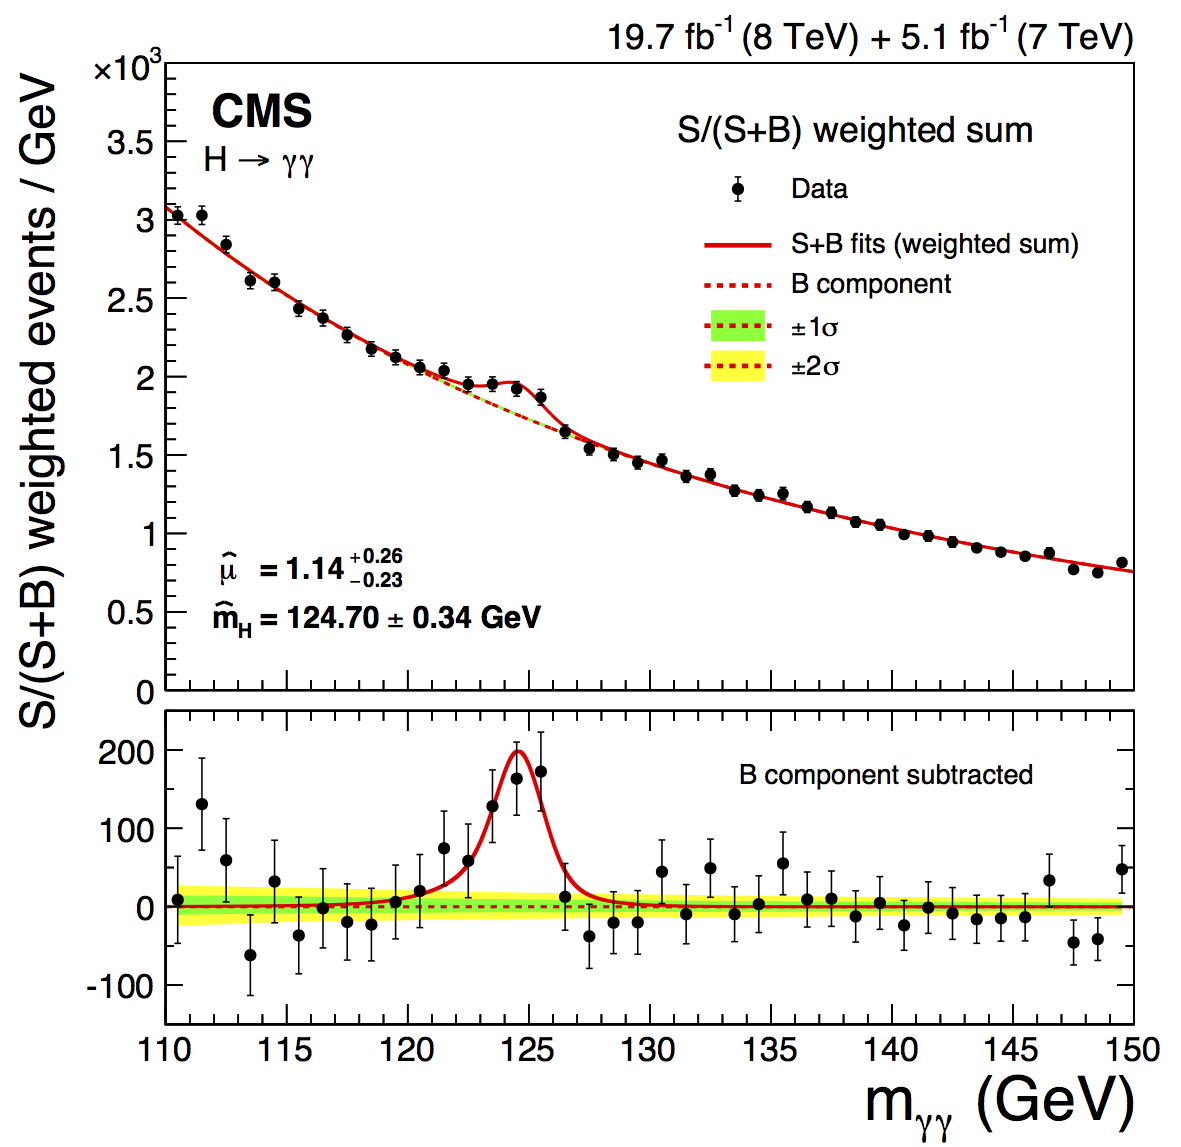
\includegraphics[width=0.6\linewidth]{Figures/higgsmeasurement.png}
\caption{Two photon invariant mass distributions from the CMS detector in 2012~\cite{CMS_Higgs_Discovery}. The peak at $125.1\GeVcc$ is the Higgs boson.}
\label{fig:higgs}
\end{figure} 


After an upgrade that ended in 2015 the LHC is now capable of producing particle collisions at energies never before achieved. The LHC has also increased its rate of collisions. To be able to gather usable data from these higher energies and collision rates the detectors on the LHC need to be upgraded as well. The Compact Muon Solenoid (CMS), one of the detectors on the LHC, is currently undergoing several upgrades. Chapter~\ref{chap:LHC_CMS} will discuss the details of the LHC and the CMS detector. Chapters~\ref{chap:test} and \ref{chap:sim} will discuss the work I did for the CMS detector outlining the analysis done on new electronics that were installed in the detector during the winter of 2018 as a part of the upgrades



\chapter{Large Hadron Collider and Compact Muon Solenoid}
\label{chap:LHC_CMS}

\section{The Large Hadron Collider}

%Talk about basics of LHC circumfrance, energies, location... and other basic stuff to intro before this paragraph which kind of does staright into details.

The LHC is located at CERN near Geneva, Switzerland. It has a circular shape and is 27 kilometers in circumference. It is about 100 meters underground and as shown in ~\ref{fig:LHC} it simply goes right under the towns and farmland in the area. To look for undiscovered particles the LHC collides protons at really high energies. After the recent upgrade the LHC now collides protons with a center of mass energy of 13 TeV, meaning the individual protons each have 6.5 TeV of energy. The theory of special relativity says that a particle can only approach the speed of light. As the protons in the LHC are traveling close to the speed of light it is more useful to use their energy rather than their speed. In addition, mass is often put into units of energy of the speed of light squared making the mass to energy conversion simple. 

\begin{figure}
\centering
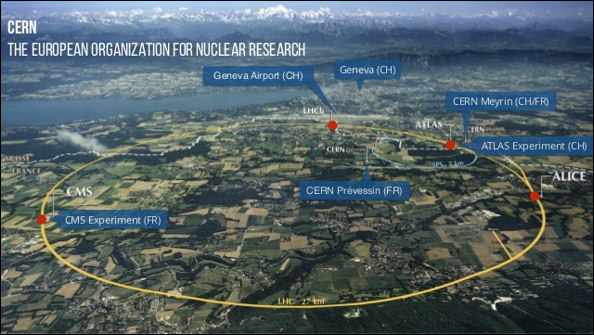
\includegraphics[width=0.8\linewidth]{Figures/LHC.png}
\caption{A picture of the LHC (outlined in yellow) with the different detectors highlighted}
\label{fig:LHC}
\end{figure}

The process the Large Hadron Collider (LHC) uses sounds simple when put into common terms. It accelerated protons to speeds very close to the speed of light and collides them in the center of a detector to see what comes out of these collisions. However actually doing this is not simple at all. To start this entire process electrons are stripped off of hydrogen gas supplying the protons for the LHC. After this the protons are put into a series of different accelerator each designed to accelerator to protons to higher and higher energies. The first accelerator is the Linac2 linear accelerator, which gets the protons up to 50 MeV. Then they are sent to the Proton Synchrotron Booster which can push them to 1.4 GeV, after which the Proton Synchrotron ring accelerates the protons to 25 GeV. At this point the protons are sorted to control the frequency at which the collisions will occur. The protons are sorted into bunches such that a proton bunch passes by every 25ns. Each bunch has about 100 billion protons in it. After sorted into these bunches the protons are sent to the Super Proton Synchrotron where they achieve an energy of 450 GeV. Finally, the protons are fed into the LHC where they will be accelerated to their highest energy. An illustration of all of these accelerators is shown in figure~\ref{fig:acceleratorcomplex}.

\begin{figure}
\centering
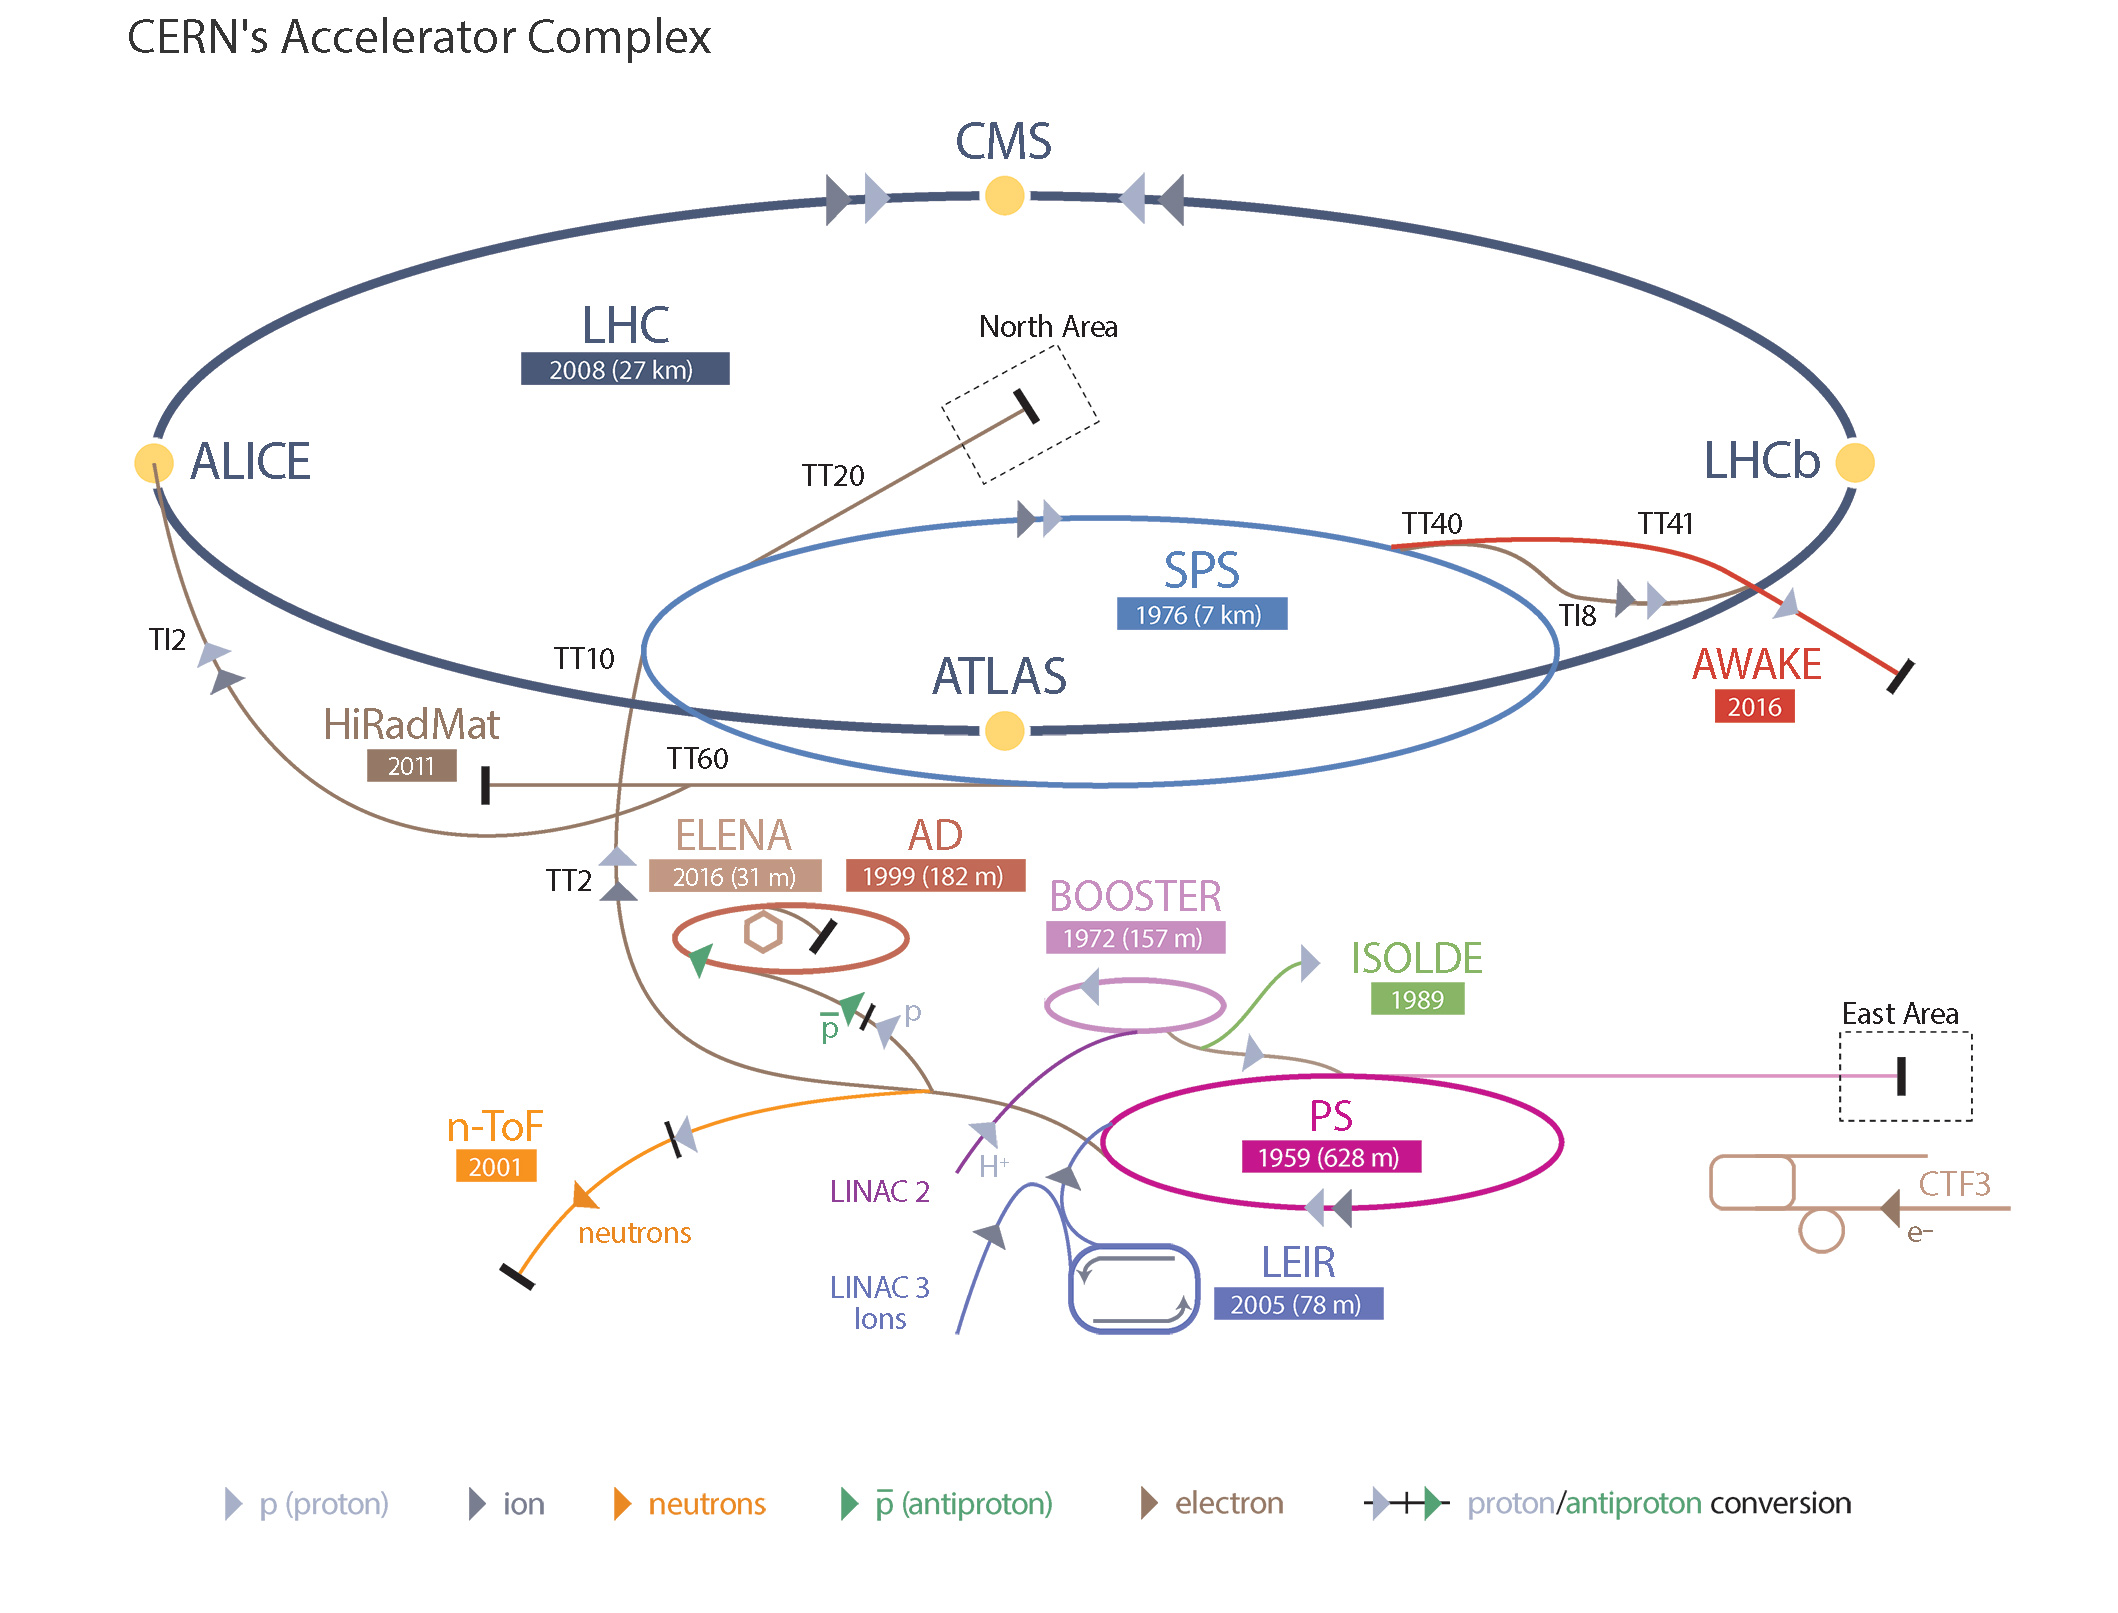
\includegraphics[width=0.8\linewidth]{Figures/acceleratorcomplex.jpg}
\caption{Chain of accelerators feeding into the LHC}
\label{fig:acceleratorcomplex}
\end{figure}

When the LHC has accelerated its particles to its peak energy it collides the particles in the middle of four different detectors. LHCb, ALICE, ATLAS, and CMS are the names of the four detectors that were built to study collisions supplied by the LHC. The CMS detector is the one I worked on during my undergraduate career, and is discussed in detail below.

\section{The CMS Detector}
The CMS detector is designed to detector particles coming out of the proton-proton collisions supplied by the LHC~\cite{CMS}. As many different types of particles come out of these collisions the CMS detector is split up into several different sub-detectors. Going from the closest to the collision point outward, first is the silicon tracker. This is responsible for measuring the total energy of the particles in the detector which is important for reconstructing the events using conservation of energy. Next is the Electromagnetic Calorimeter which is responsible for detecting a myriad of charged particles such as photon, and electrons. Then there is the Hadron Calorimeter which is responsible for detector hadrons, which are particles made up of quarks, such as protons neutrons and pions. These calorimeters work by covering the possible directions out of the collision with scintillator tiles. When the particles hit these tiles they lose some of their energy depositing light proportional to the energy of the particle. The particle will eventually stop having lost all of its energy giving us a reading on its total energy. Finally, are the muon chambers. Muons are interesting particles because while they are heavy particles that will decay they have long enough lifetimes to make it through the detector. In addition, they tend to not be stopped by the detector like the two prior calorimeters almost always stop the particles they detect. Since there is a magnetic field encompassing the detector and the muons have a charge they will curve as they pass through the muon chambers. While not completely stopping the muons will give a reading in the chambers showing its path of travel. By measuring the curve of this path of travel we can measure the momentum. By combining the the data from all the different sub detectors we can get a picture of almost all of the particles that came out of the collision. There are exceptions such as neutrinos which tend to pass through anything leaving no trace. Nevertheless we are able to use this to recreate what exactly came out of the collision, which allows us to find evidence of particles like the top quark which decays so quickly it does not even make it to the detector.

The CMS detector is designed to detector particles coming out of the proton-proton collisions supplied by the LHC. As many different types of particles come out of these collisions the CMS detector is split up into several different sub-detectors. Going from the closest to the collision point outward, first is the Silicon Tracker. The Silicon Tracker is capable of finely measuring the path of the particles that go through it. The CMS detector produces a 4 Tesla magnetic field throughout most of the detector. As charged particles move through the magnetic field, their path curves. The Silicon Tracker allows us to measure the curvature of their path and find their momentum. Next is the Electromagnetic Calorimeter which is mainly responsible for measuring the energy of photons and electrons that come out of the collision. Then there is the Hadron Calorimeter (HCAL) which is responsible for detector hadrons, which are particles made up of quarks, such as protons neutrons and charges pions. The HCAL works but covering almost all $4\pi$ direction out of the collision with scintillator tile. When particles go through the scintillator tile they interact with the molecules exciting them while the particles lose some of their energies. The molecules in the scintillator will then go back to their original energy state emitting a photon. These photons are gather by an optical fiber. By counting these photons we can measure the energy lost by the particle. The detector has enough scintillator tile in the path of the particle to make it highly probably the particle will lose all of its energy in the detector. While this is still a simplification of the process counting the number of photons from the scintillator tile is the basis of the measurement of the energy of the particle. Finally, are the Muon Chambers. Unlike other particles the muon tends to just go through the scintillator only losing a small portion of its energy. This means the muons will reach the last section of the detector mostly unperturbed. Since the muons are charges their path will be curved by the magnetic field so their momentum is measured by a process similar to that of the Silicon Tracker. An illustration of the of the different sub-detectors and the particles that will interact with them is shown in figure~\ref{fig:CMSlayout}.

Even with all of these sub-detector there are still particles not directly detected. Neutrinos for example tend to go through everything without interacting so they do not appear in our detectors signals. Several of the particles on table~\ref{tab:particles} decay before even reaching the detector. To find evidence of these particles we have to find indirect evidence of them. The top quark for example nearly 100\% of the time decays into a bottom quark and a W boson. The W boson then either decays into a charged lepton neutrino pair or a light quark anti-quark pair. By finding evidence of these particles in close proximity we can deduce these came from a top quark.

\begin{figure}
\centering
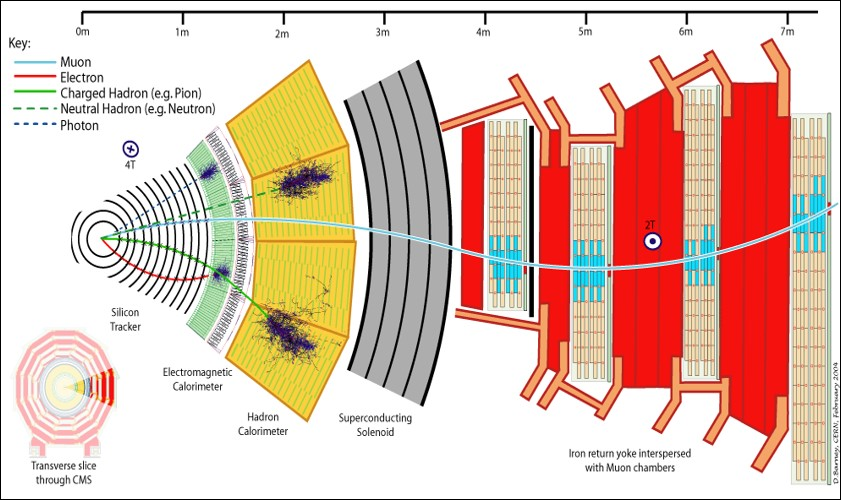
\includegraphics[width=\linewidth]{Figures/CMSlayout.jpg}
\caption{A slice of the CMS detector highlighting the different sub-detectors and showing different particles and where they are stopped}
\label{fig:CMSlayout}
\end{figure}

\subsection{Hadron Calorimeter}
One of the main jobs of the calorimeter is to measure the energy of the of the incident particle. When the particle hits the scintillator tile and loses energy it emits photons into the tile proportional to the amount of energy it lost. In order to collect these photons a optical fiber is put in the outer edge of the tile. A picture of the scintillator tile is shown in figure~\ref{fig:Tile}. This fiber will capture the photons and channel them to a photo detector, which will take the light signals and convert them to charge signals. The original photo detector for the HCAL was the hybrid photo-diodes (HPD) but they are being replaced by silicon photomultipliers as apart of some of the upgrades on the CMS detector. 

\begin{figure}
\centering
\includegraphics[width=0.6\linewidth]{Figures/Tile.png}
\caption{A picture of a scintillator tile with the optical fiber around the edges.}
\label{fig:Tile}
\end{figure}


There are three main section to the HCAL. There is the Hadron Barrel (HB)~\cite{HB}, which surrounds the beam-line like the edge of a cylinder, the Hadron End-cap (HE), which caps off the cylinder made by HB. These two parts make a cylinder which has the beam-line going through the center and the collision point in the center. Lastly there is the Hadron Front-cap (HF) which is shaped like HE but is located much further away from the collision point~\cite{HF}. To describe the geometry of the detector we use a coordinate system related to spherical coordinates with the origin being the collision point and polar angle of 0 being along the beam-line. Phi is the azimuthal angle and Eta is related to the polar angle by $\eta = -\ln(\tan(\theta/2))$ which gives a value of 0 perpendicular to the beam-line and $\pm\infty$ along the beam-line. Usually these coordinates are arranged into discrete integers values denoted iphi and ieta, which are arranged such that a scintillator tile covers one ieta and one iphi as shown in figure~\ref{fig:Depth} but there are exception to this. For the distance from the beam-line depth is used which is also a discrete value but there are often more than one scintillator tiles in a single depth. 


\begin{figure}
\centering
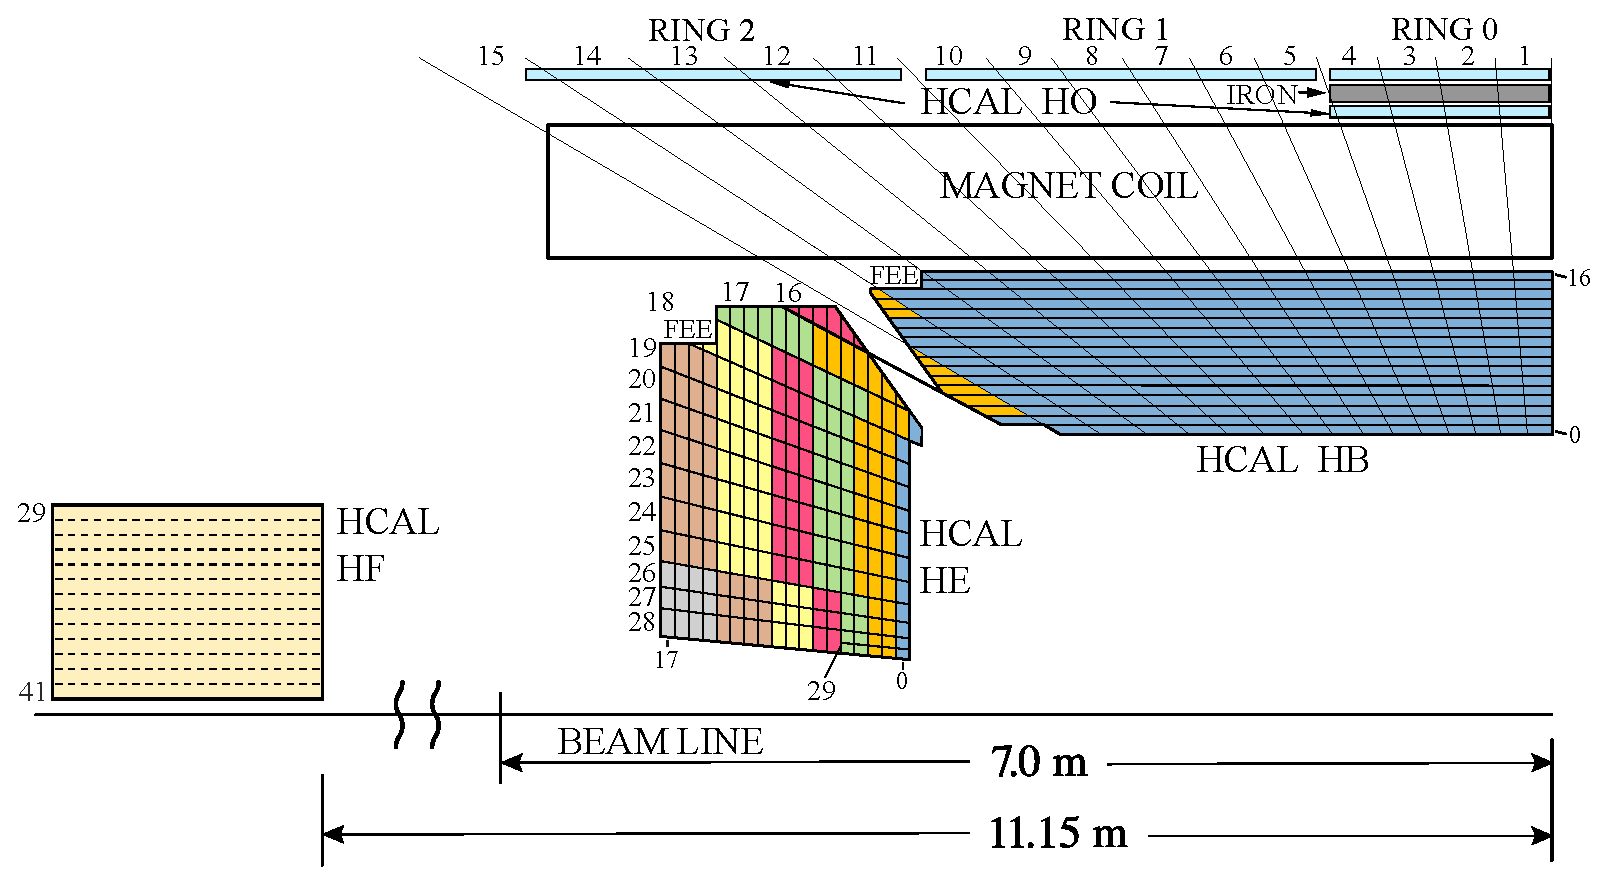
\includegraphics[width=\linewidth]{Figures/Depthsegmentation.pdf}
\caption{Layout of the HCAL showing a single iphi slice of HE HB and HF. Each box represents a scintillator tile}
\label{fig:Depth}
\end{figure}

\subsection{Silicon Photomultipliers}
The SiPM does its job of counting the photons from the scintillator by shining them on a pixel face. This is just a circular array of really small pixels. A picture of the SiPM is in figure~\ref{fig:SiPM} showing several pixel faces. There are about 33000 pixels on a 3.3 mm diameter pixels face. When an individual photon hits one of the pixels on the pixel face it causes a capacitor to fire off a particular amount of charge. The total output charge of the SiPM is the sum of all of the pixels output charge. Theoretically one just needs to sum up the total amount of output charge of the SiPM and one can count the number of incident photons since each pixel will fire off a set amount of charge. The counting of the number of incident photons will give a measurement of the incident particles energy. There are some things that make the SiPMs reading not so simple. SiPMs are non-linear devices meaning the total output charge of the SiPM does not necessarily increase linearly with the number of incident photons. In fact, experiments have shown that graphing the number of incident photons vs the SiPM output charge it looks more like a square root function rather than a straight line. At low incident photon count on the order of 1000 photons the SiPM is very close to a linear device but as the incident number of photons increases the output charge does not increase at the same rate. There are several factors that contribute to SiPM non-linearity but the two main ones are cross talk and saturation. Cross talk is when a pixel is activated by a photon there is a chance that this activated pixel could activate some of its neighboring pixels artificially increase the output charge of the SiPM. When the photon hits a pixel it excites an electron causing an electron cascade and charge to flow. This excited electron has a chance to emit an IR photon which could go in any direction. If it hits one of the neighboring pixels it could activate it just like an incident photon. 

Saturation is when a pixel is hit in rapid succession by multiple photons. When a pixel is hit by a photon it discharges its capacitor which is the source of its output charge. After the pixel fires it needs some time on the order of 10 nanoseconds to recharge its capacitor. If the pixel is hit it simply fires off whatever charge it has in its capacitor at the time which could be reduced from its normal charge. Given that the SiPM has about 33000 pixels on its pixel face, when the number of incident is on the order of 1000 this effect is insignificant, but particles can produce much more photons where this effect can be much more significant. The non-linear properties of the SiPM makes it a bit harder to get accurate measurements, but there are ways to study them which will allow us to compensate for these affects.

\begin{figure}
\centering
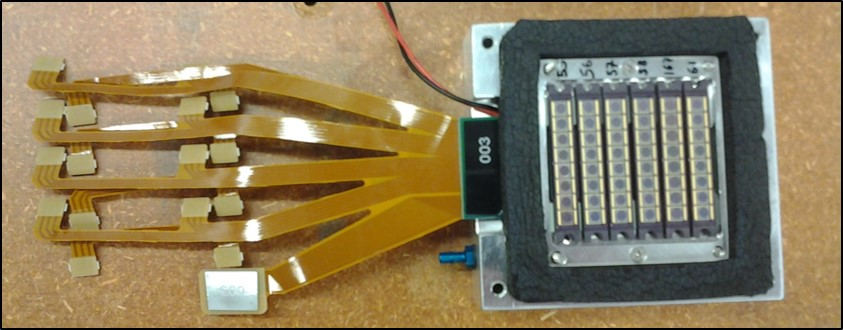
\includegraphics[width=\linewidth]{Figures/SiPM.jpg}
\caption{A picture of a Silicon Photomultiplier}
\label{fig:SiPM}
\end{figure}






\chapter{Analysis}
\label{chap:ana}
\section{SiPM Simulation}

In addition to studying the new electronics with the test beam, we also did some work wtih a SiPM simulation which could use theoretical signals from the detector and give the SiPM's response to them. When the light from the detector goes to the SiPM a Y11 light mixer is used so that the light is spread across the pixel face. The light mixer has a unique shape, shown in figure ~\ref{fig:Y11} in which it shines the light onto the pixel face. Using a mathematical representation of this pulse shape we can simulate how light is shined on the pixel face. We can then create a virtual pixel face that has accurate geometric representation. Each of these virtual pixels could be activated by the incoming Y11 light pulse and would respond by firing off a set amount of charge as would an actual SiPM. When these pixels are activated they also have a certain probability to activate a neighboring pixels which will simulate the cross talk of the SiPM. Each pixel also has a recharge rate such that if hit in rapid succession it will fire with a reduced amount of charge emulating the saturation effect. Using this simulation we easily adjust the number of input photons and get very good details of the SiPM response. We can also easily turn different things off to see how significant individual effects are. This simulation is capable of producing more fine tuned data and in greater quantities than test beam data. In addition, it is able to simulate situations that are not possible in the test beam. On the other hand the accuracy of this simulation is heavily dependent on the data we input into it.

Since the program can simulate the non-linearity effects of the SiPM, we can use theoretical inputs to the SiPM to study its effects. The light a particle deposits in a scintillator tile can vary in time the Y11 light mixer ensures that the input light pulse shape remains constant. This means to change energy of the incident particle we just have to increase the number of photons in the input pulse while keeping the same shape. The output of the virtual SiPM is normalized so if the simulation was a completely linear device its output "charge" should exactly equal the number of input photons. 

\begin{figure}
\centering
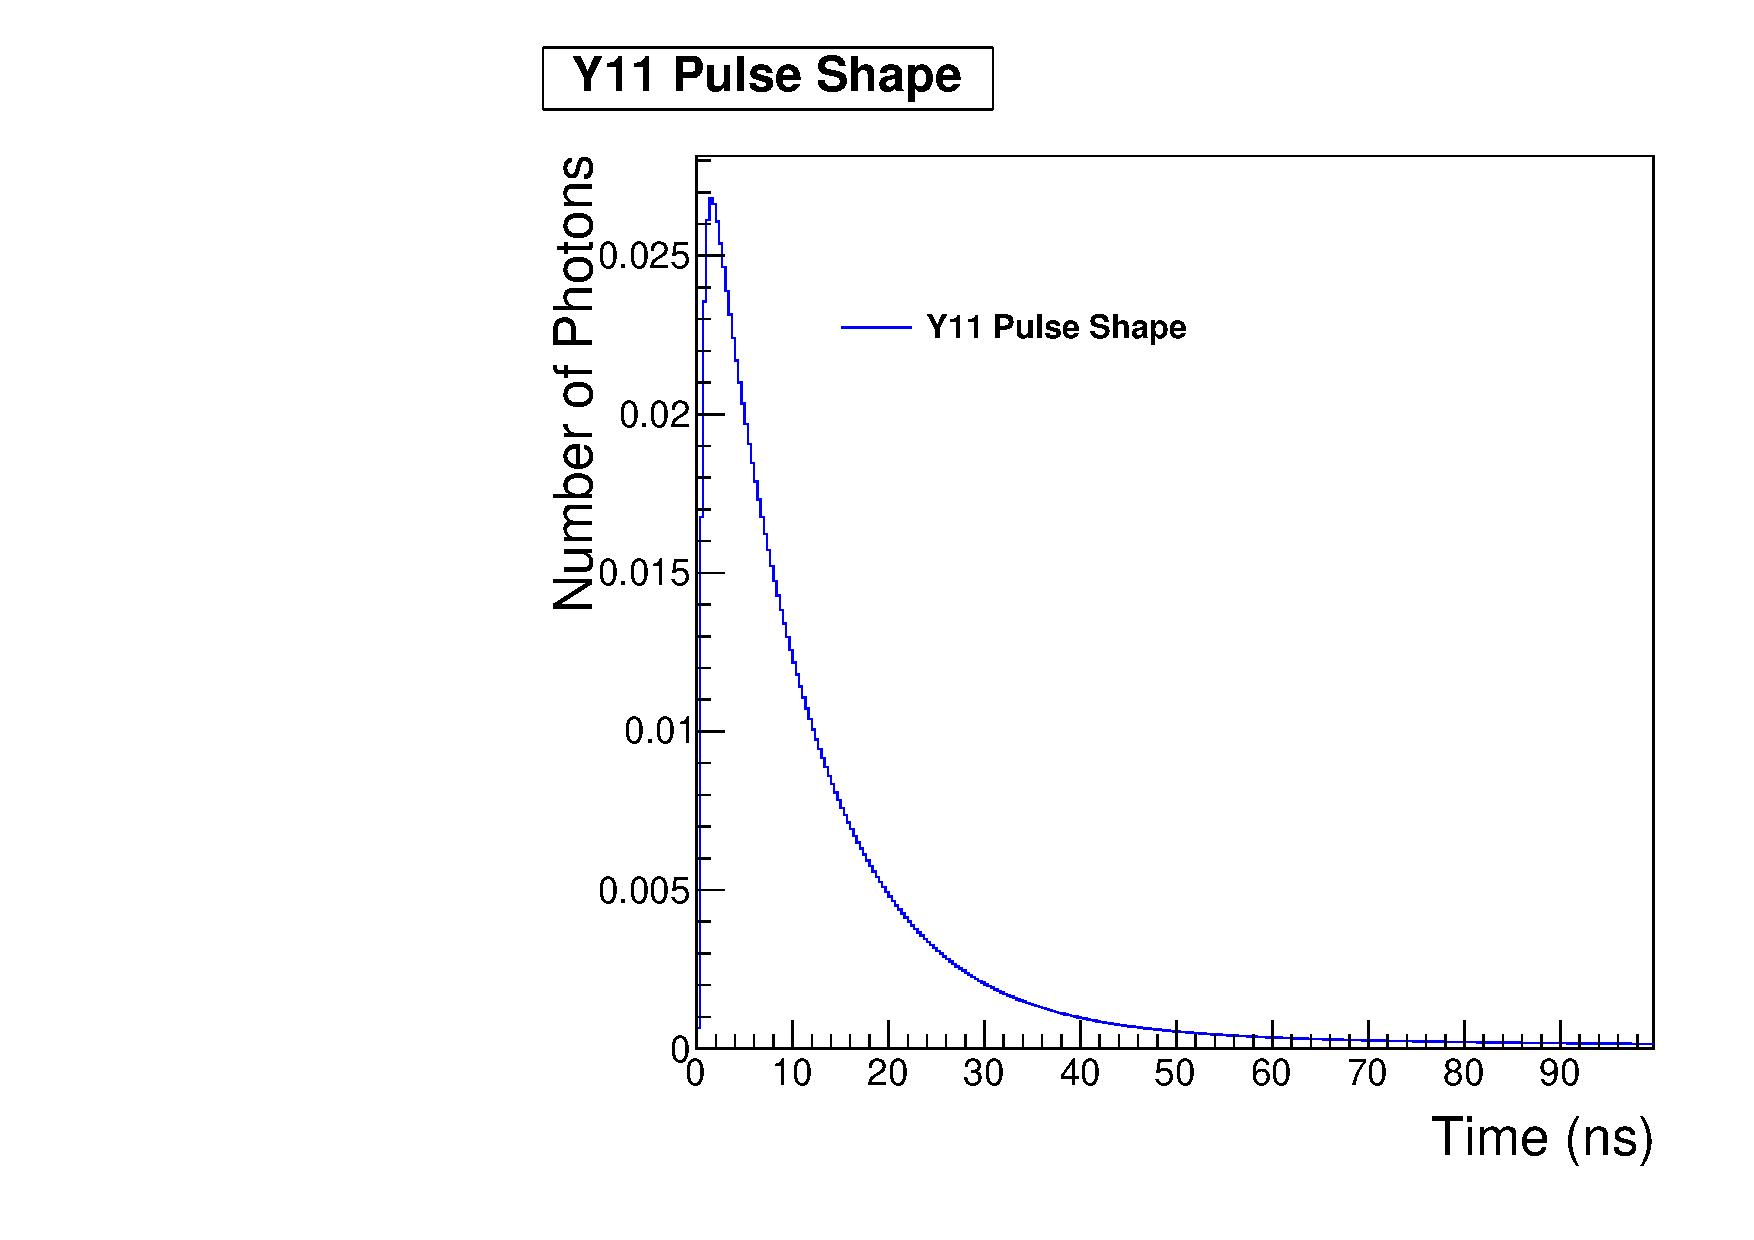
\includegraphics[width=0.8\linewidth]{Figures/Y11.pdf}
\caption{A graph of the Y11 pulse shape with nanoseconds on the x axis and number of incident photons on the y axis}
\label{fig:Y11}
\end{figure}

\section{Simulation Analysis}

To do the analysis using the SiPM simulation, we simply measure the total output of the SiPM over a light pulse and compare it to the number of input photons. Since there is a degree of randomness we will use the average pulse over several inputs. Compared to using test beam data the analysis with the simulation is simple. In test beam the energy of the particle is spread over several SiPMs while in the simulation we have a very fine control of the input energy to the single SiPM. With a plot of input number of photons vs SiPM output charge we then create a correction curve that is necessary to make the graph linear. This is process for doing a non-linearity analysis using test beam data so we can compare the two correction curves to see if there is agreement. With other analyses it is common to simply divide out the cross talk. Given that there is a $15.4\%$ chance of crosstalk with a large signal of several thousand photons it is assumed that $15.4\%$ of the signal from the SiPM is due to cross talk so that number is simply divided out. This means the majority of the effects that the correction curve is compensating for is saturation. Figure~\ref{fig:SimNon} shows the non-linearity obtained from the simulation.

\begin{figure}
\centering
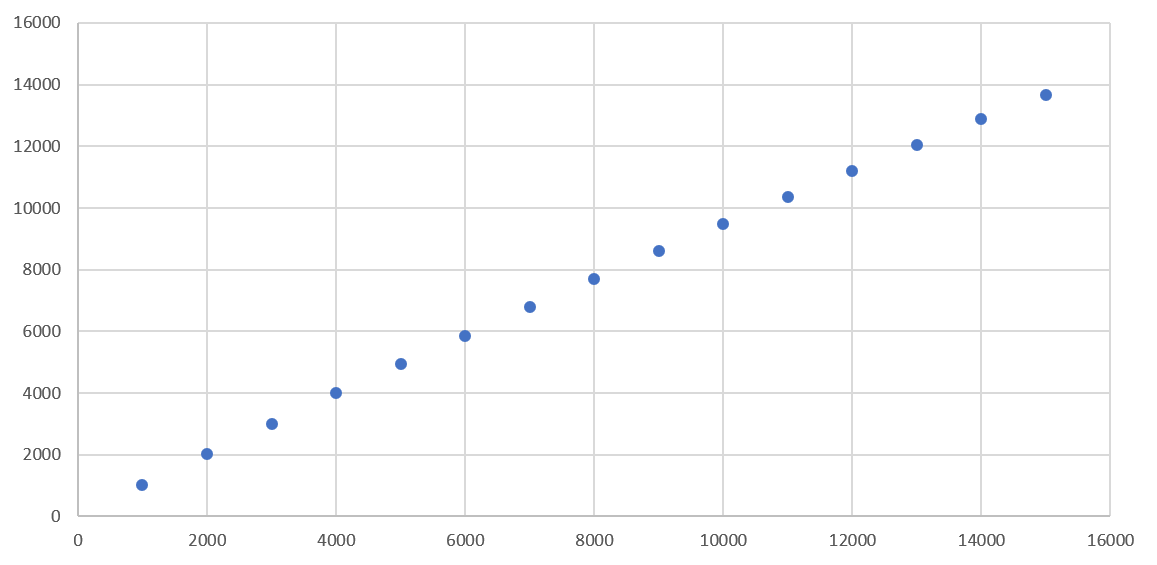
\includegraphics[width=0.8\linewidth]{Figures/SimNon.png}
\caption{Graph of number of incident photons vs output charge of the SiPM simulation with a y=x line for reference. Given the units of the simulation a perfectly linear device would have all data points falling on the y=x line but as shown as the number of incident photons is increased the data points fall short of this line.}
\label{fig:SimNon}
\end{figure}

To be sure the simulation is designed correctly it is useful to compare things like non-linearity to the actualy SiPM. Figure~\ref{fig:NonLin} shows the non-linearity of the SiPM from shining a laser directly on the SiPM. Figure~\ref{fig:Cor} shows a similar plot constructed using the simulation. There is significant disagreement between these two sets of data.

\begin{figure}
\centering
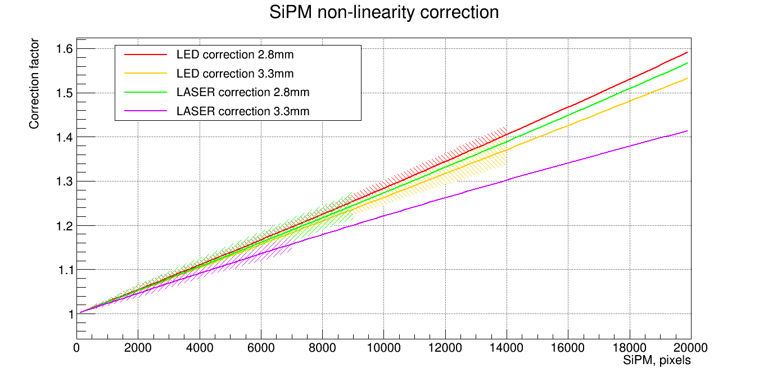
\includegraphics[width=\linewidth]{Figures/LaserNonLin.png}
\caption{Graph of the correction factor vs. number of pixels fired. The correction factor is the number the output needs to be multiplied by in order to obtain the linear output value. This means a perfectly linear device would always have a correction factor of 1. This data was obtained from shining a laser directly on the SiPM.}
\label{fig:NonLin}
\end{figure}

\begin{figure}
\centering
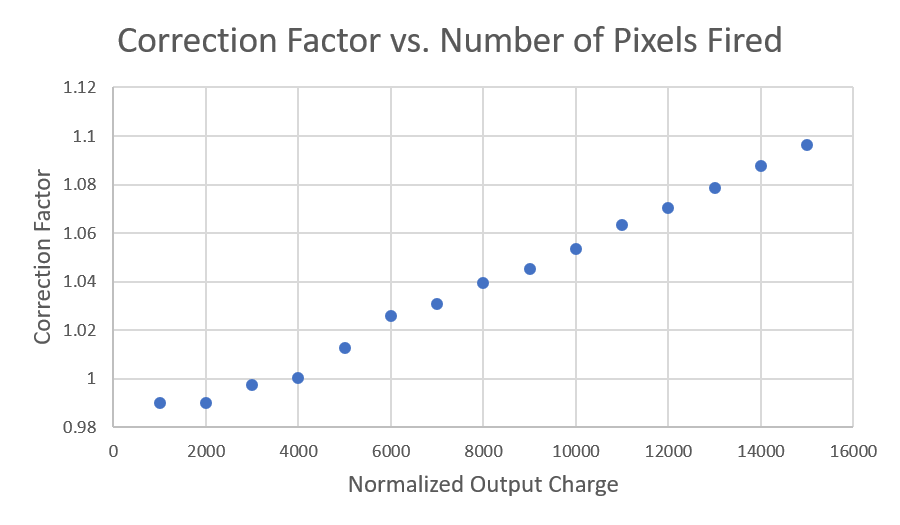
\includegraphics[width=\linewidth]{Figures/CorFac.png}
\caption{Graph of the correction factor vs. number of pixels fired. The correction factor is the number the output needs to be multiplied by in order to obtain the linear output value. This means a perfectly linear device would always have a correction factor of 1. This data was obtained from the SiPM simulation.}
\label{fig:Cor}
\end{figure}

One effect of the saturation that is less understood and harder to implement is that the pixels can sometimes recharge faster. This effect is due to the QIE chips in the readout modules which in addition to taking and processing the charge from the SiPMs also supply the charge that recharges the capacitors for each individual pixel. The capacitors for the pixels recharge exponentially like normal RC circuits. Normally the time constant for the capacitors is about 9ns which means the capacitor is completely charges after 20ns but this is when the SiPM is outputting a very low amount of charge to the QIE chips. When the SiPM is outputting more charge the QIE chips then supply more charge to the SiPM recharging the pixels faster. When the pixels recharge fast they will fire off closer to their maximum charge even when hit in rapid succession. This means as saturation becomes more prevalent with a high number of incident photons this reduces the effects of saturation. The effect of different recharge time for the pixels can be see in figure~\ref{fig:trc}.

\begin{figure}
\centering
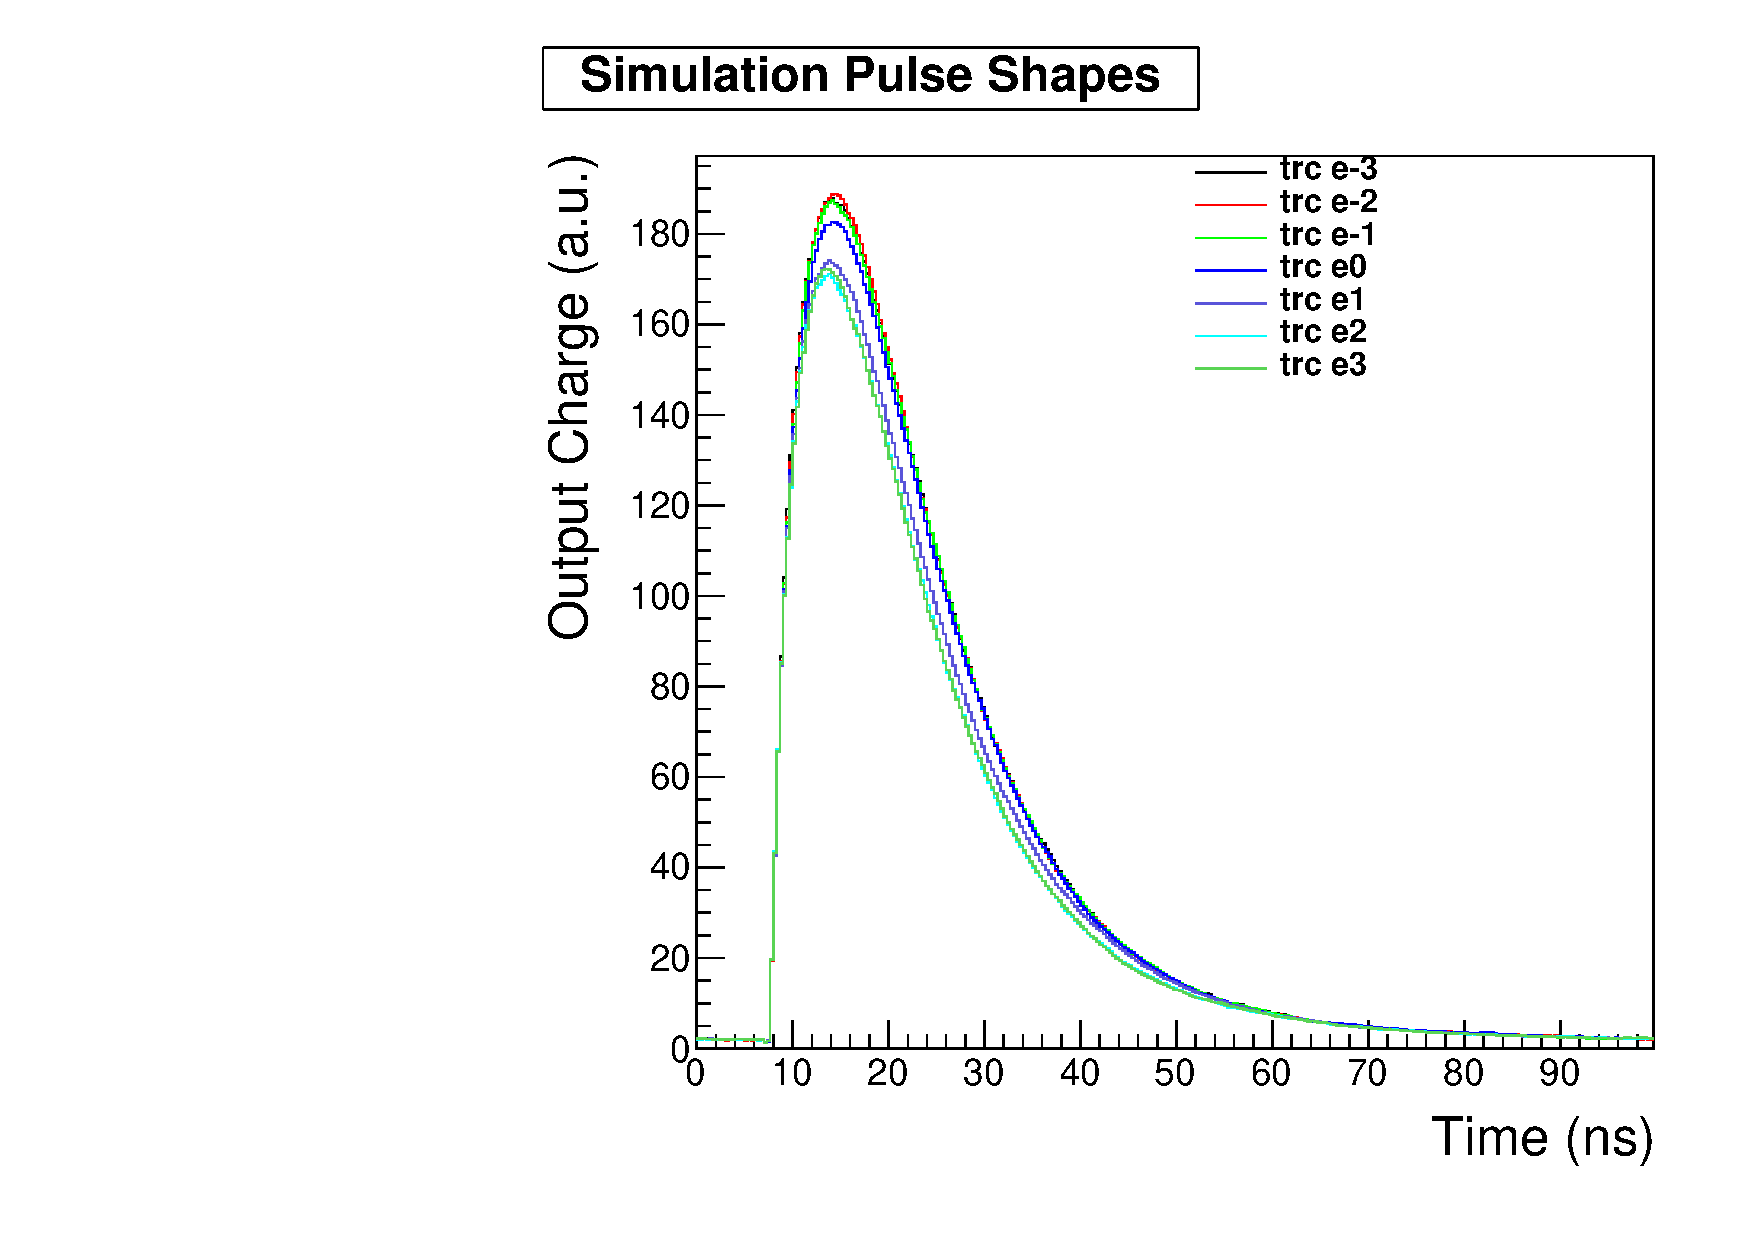
\includegraphics[width=0.8\linewidth]{Figures/trc.pdf}
\caption{Output pulses of the SiPM simulation with 1000 incidents photons comparing the effect of changing the recharge time constant on the pixels. The TRC value is the recharge time constant ranging from $10^{-3}$ to $10^3$.}
\label{fig:trc}
\end{figure}

Using the simulation we can also look at the pulse shape of the SiPM. This pulse shape should theoretically be the same obtained from test beam data. One of the main things that is necessary to look at is does the pulse shape change significantly with a change in input energy. As shown is figure~\ref{fig:SimPul} does not significantly change with different energies.

\begin{figure}
\centering
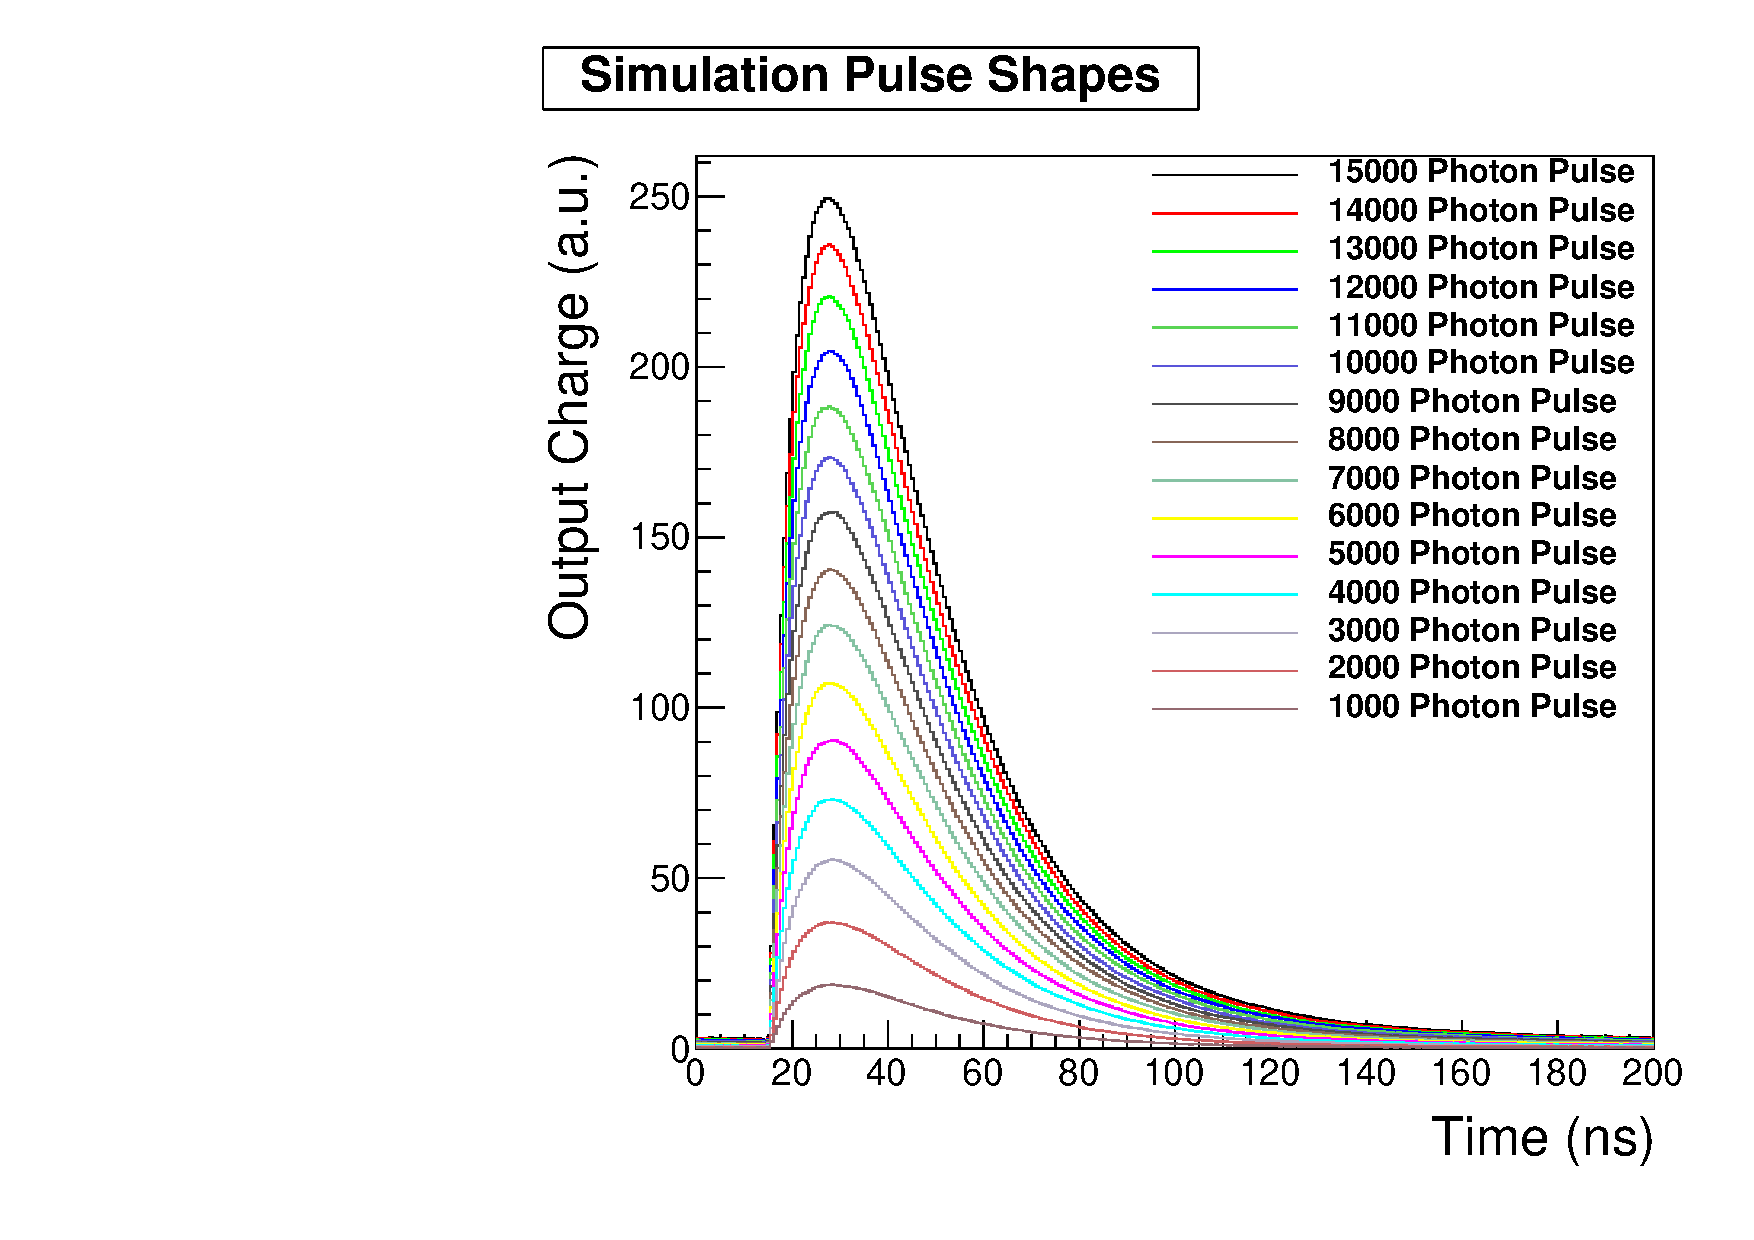
\includegraphics[width=0.8\linewidth]{Figures/SimPul.pdf}
\caption{Pulse shapes from the SiPM simulation. They are stacked on top of each other to highlight any differences from an increase input photon count.}
\label{fig:SimPul}
\end{figure}

We can compare the pulse shape from the simulation to the one obtained from test beam data. Theoretically these pulses should be the same. For comparison we simply plot the two pulse shapes on top of each other and see if there are any major differences. To minimize the interference of other effects like non-linearity we can compare pulses from similar output charge. Using the conversion ratio of 40 fC to 1 photo electron we can compare pulses from the same charge range. For instance, for the charge range 10,000-29,000 fC we compare it a pulse of 500 photo electrons from the simulation. Figures ~\ref{fig:1comparison_together}-~\ref{fig:3comparison_together} show these comparisons. While they do have the same basic shape there are some significant differences mostly the simulation is much narrower in the base.

\begin{figure}
\centering
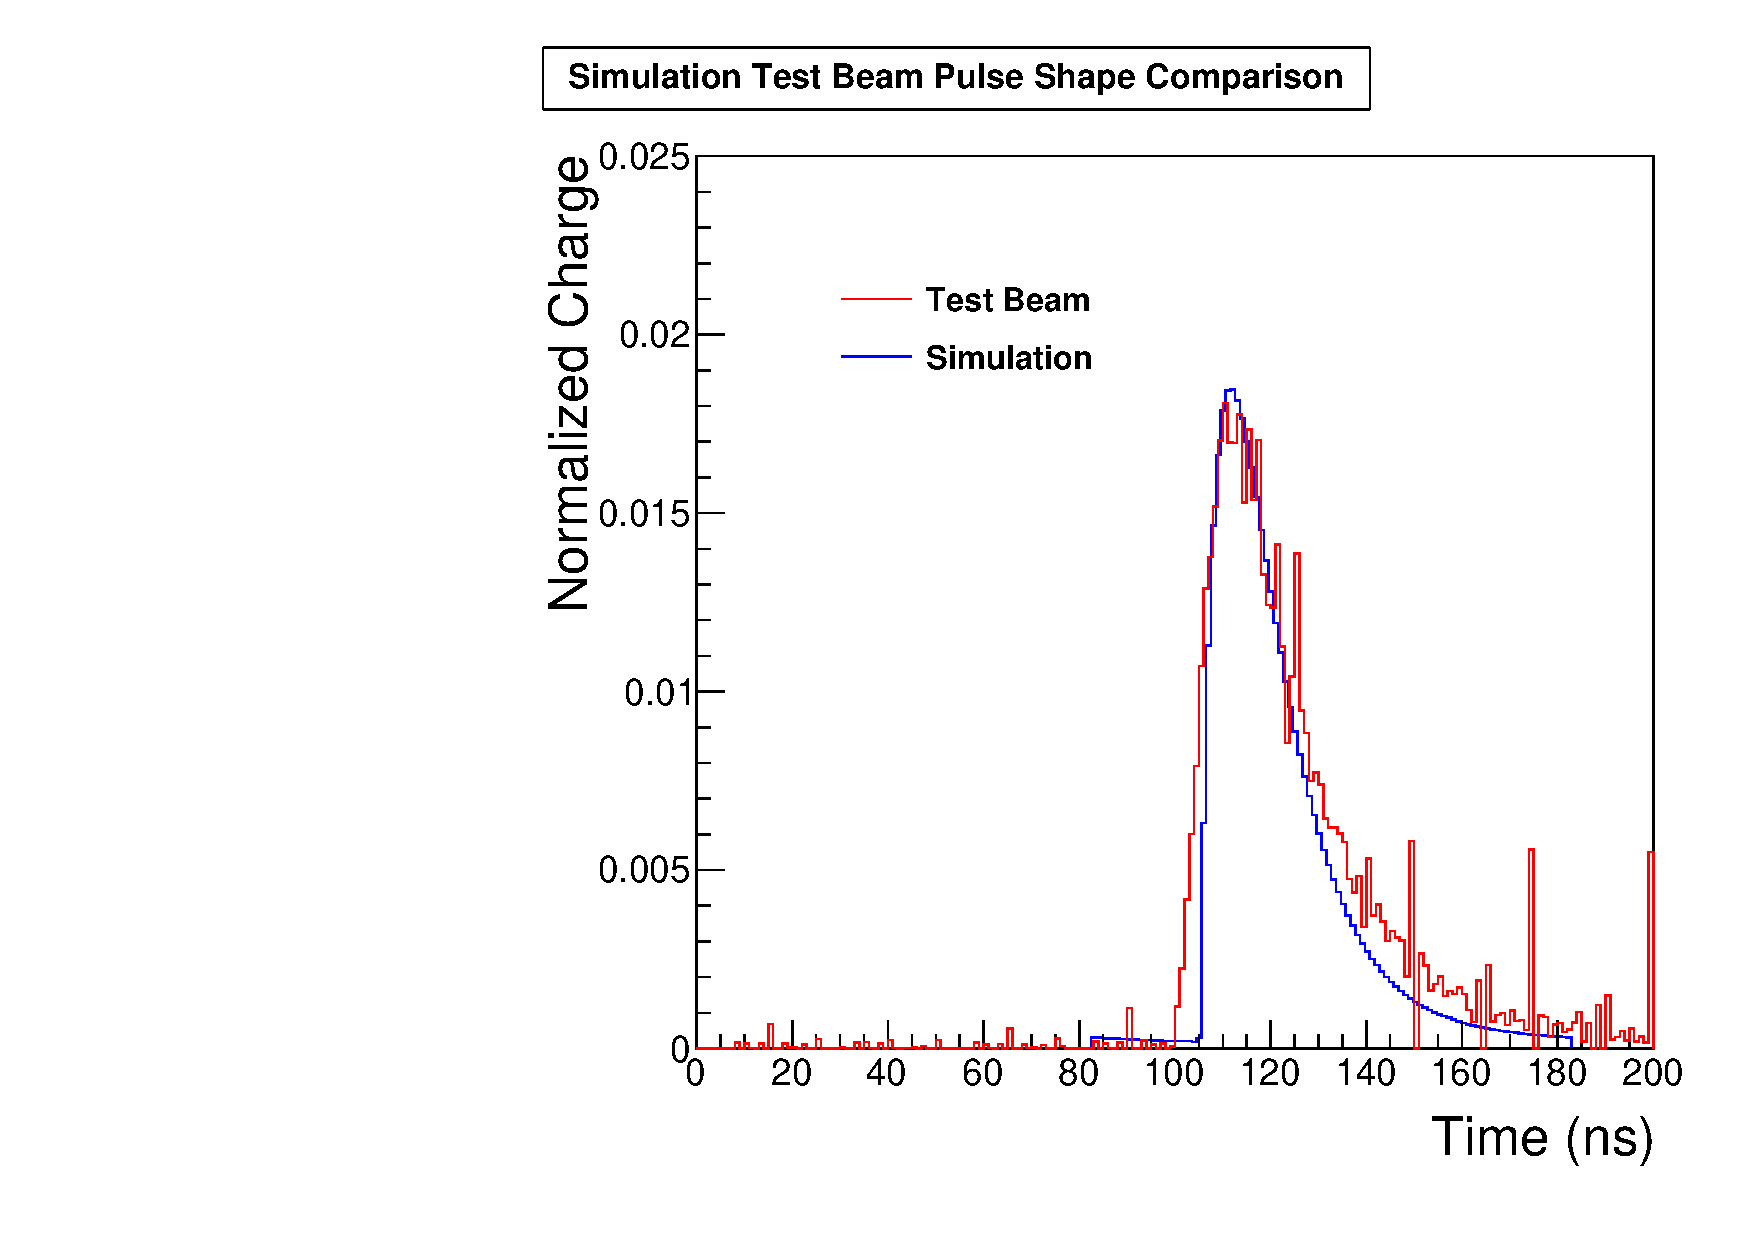
\includegraphics[width=0.495\linewidth]{Figures/10Comparison.pdf}
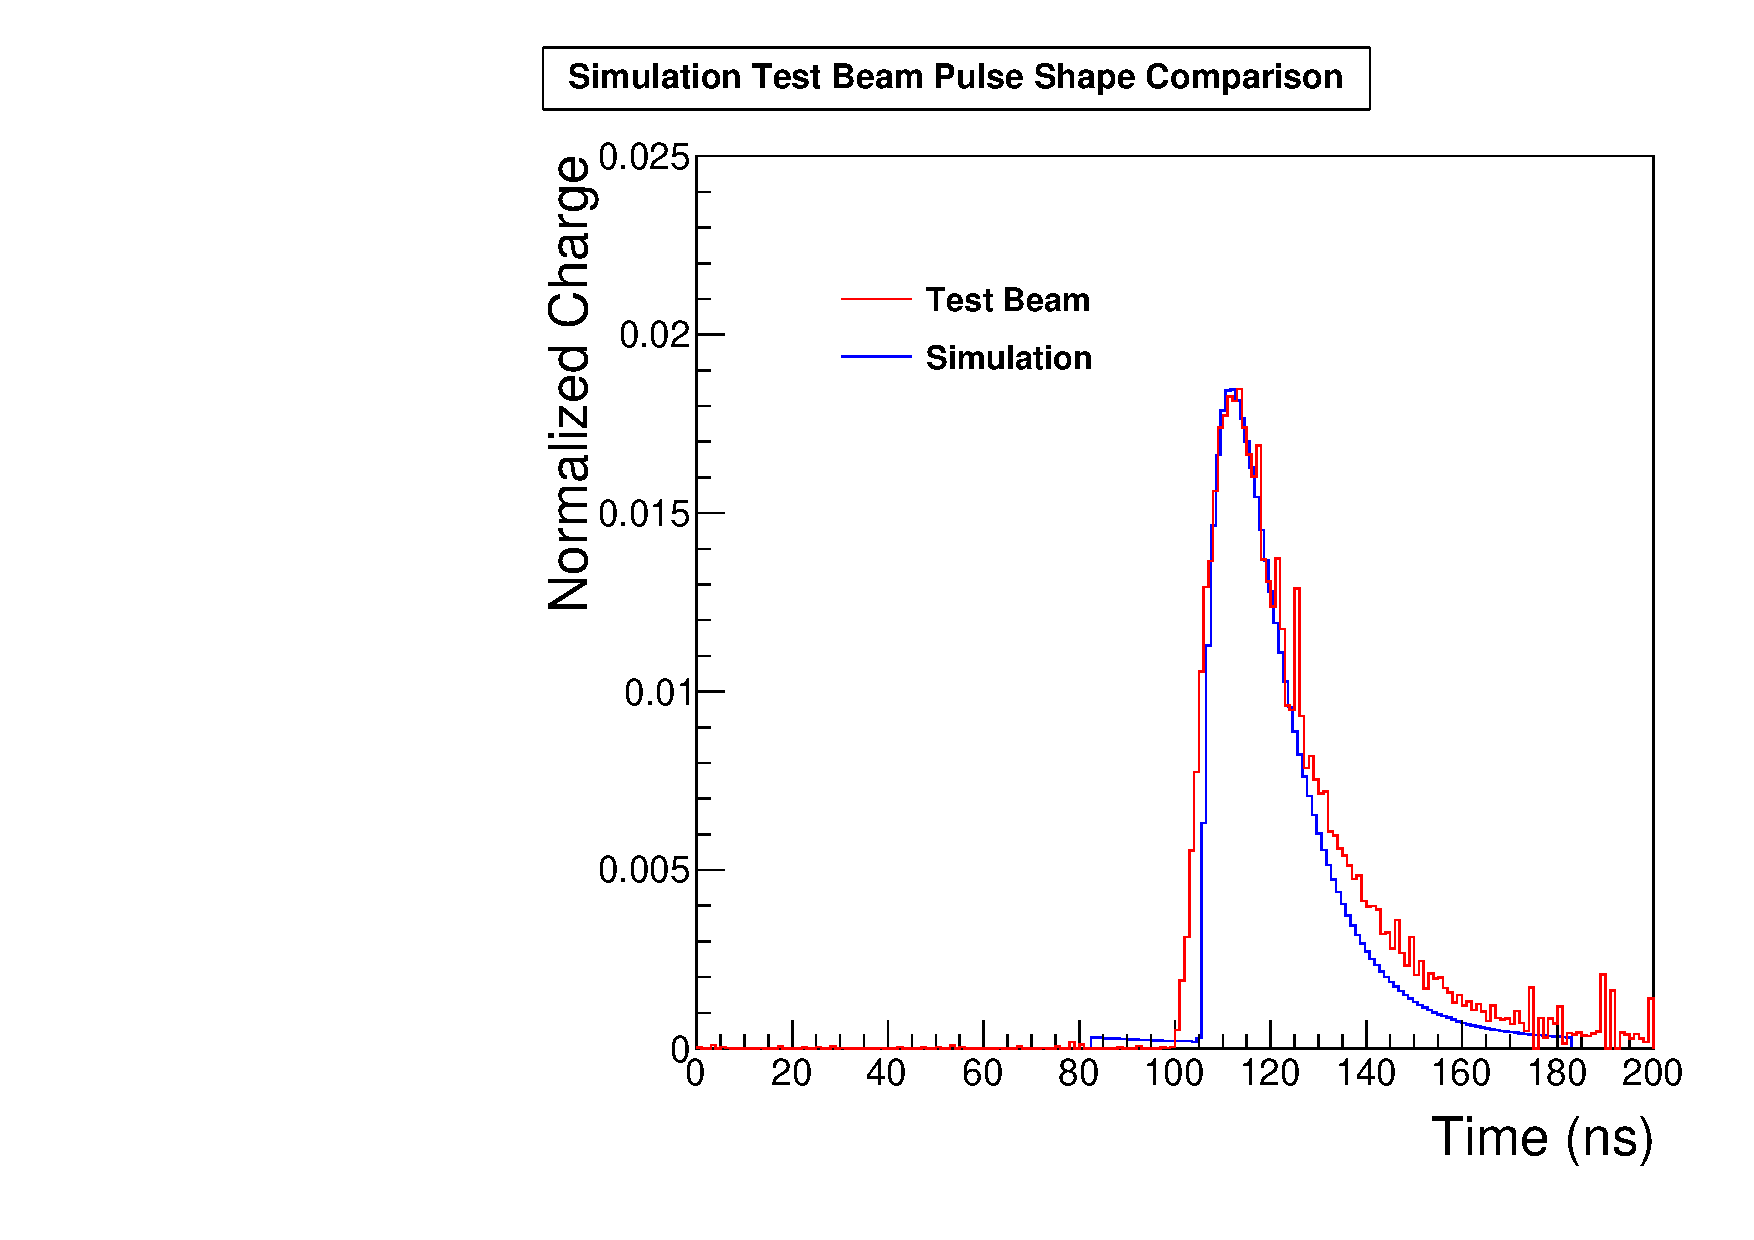
\includegraphics[width=0.495\linewidth]{Figures/29Comparison.pdf}
\caption{Histogram of the pulse shapes from the simulation and the test beam overlapping for comparison purposes. On the left the charge range is 10,000-29,000 fC on the right is 29,000-50,000 fC}
\label{fig:1comparison_together}
\end{figure}

\begin{figure}
\centering
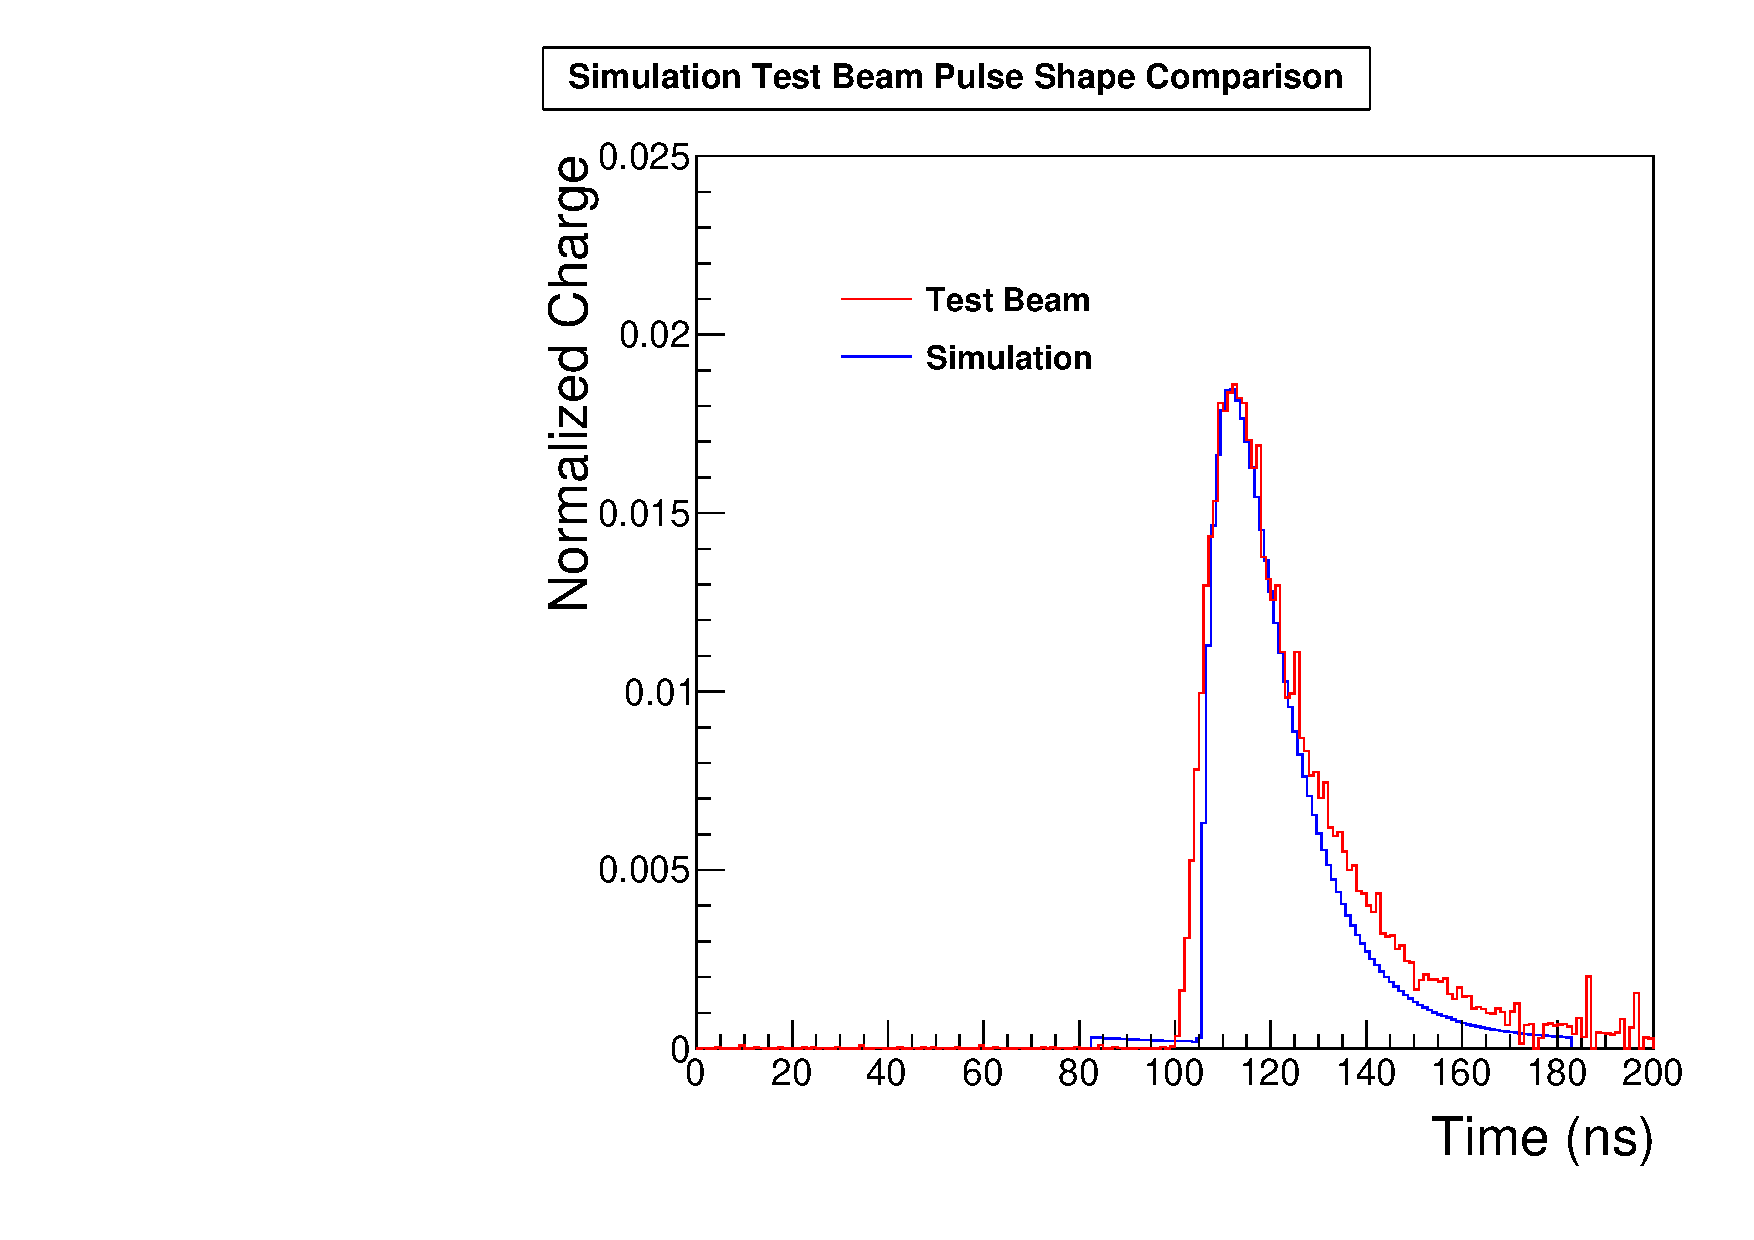
\includegraphics[width=0.495\linewidth]{Figures/50Comparison.pdf}
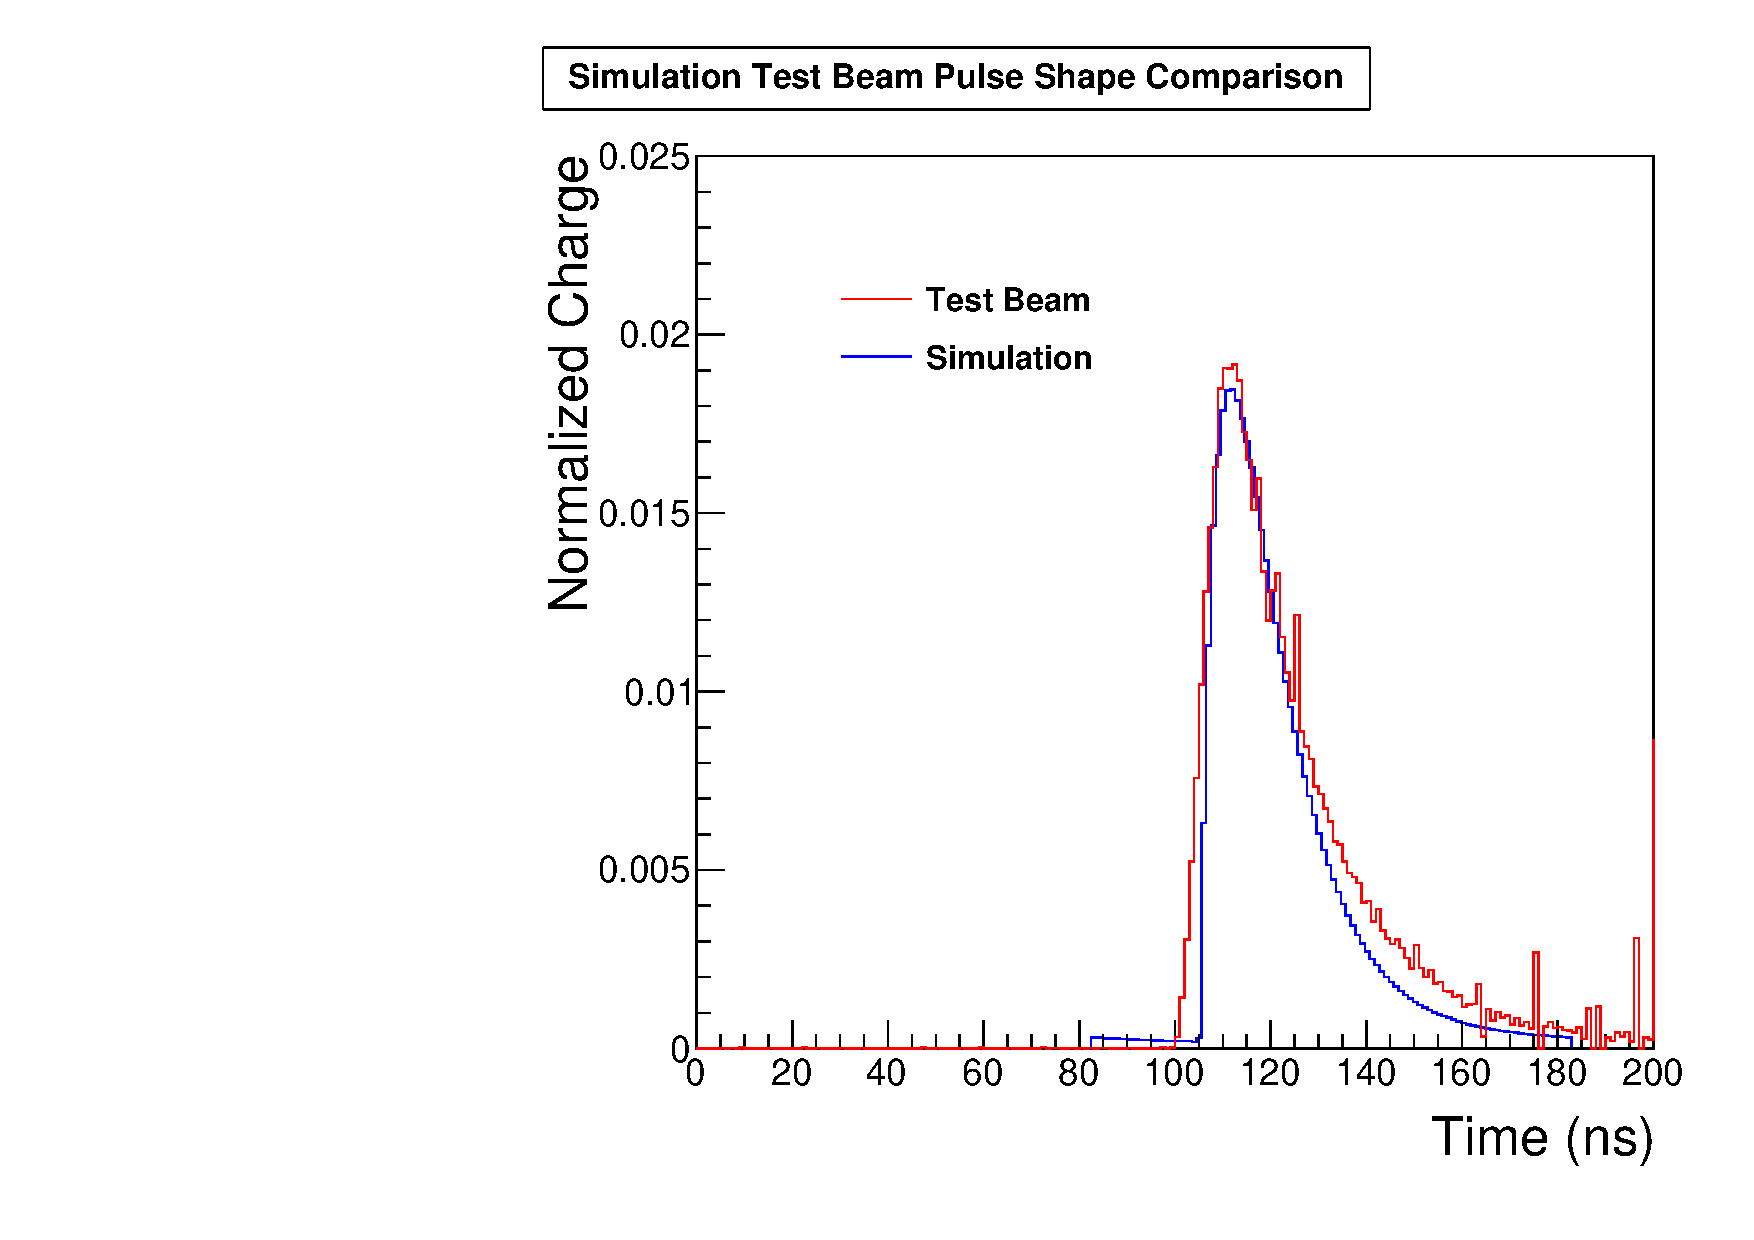
\includegraphics[width=0.495\linewidth]{Figures/80Comparison.pdf}
\caption{Histogram of the pulse shapes from the simulation and the test beam overlapping for comparison purposes. On the left the charge range is 50,000-80,000 fC on the right is 80,000-125,000 fC}
\label{fig:2comparison_together}
\end{figure}

\begin{figure}
\centering
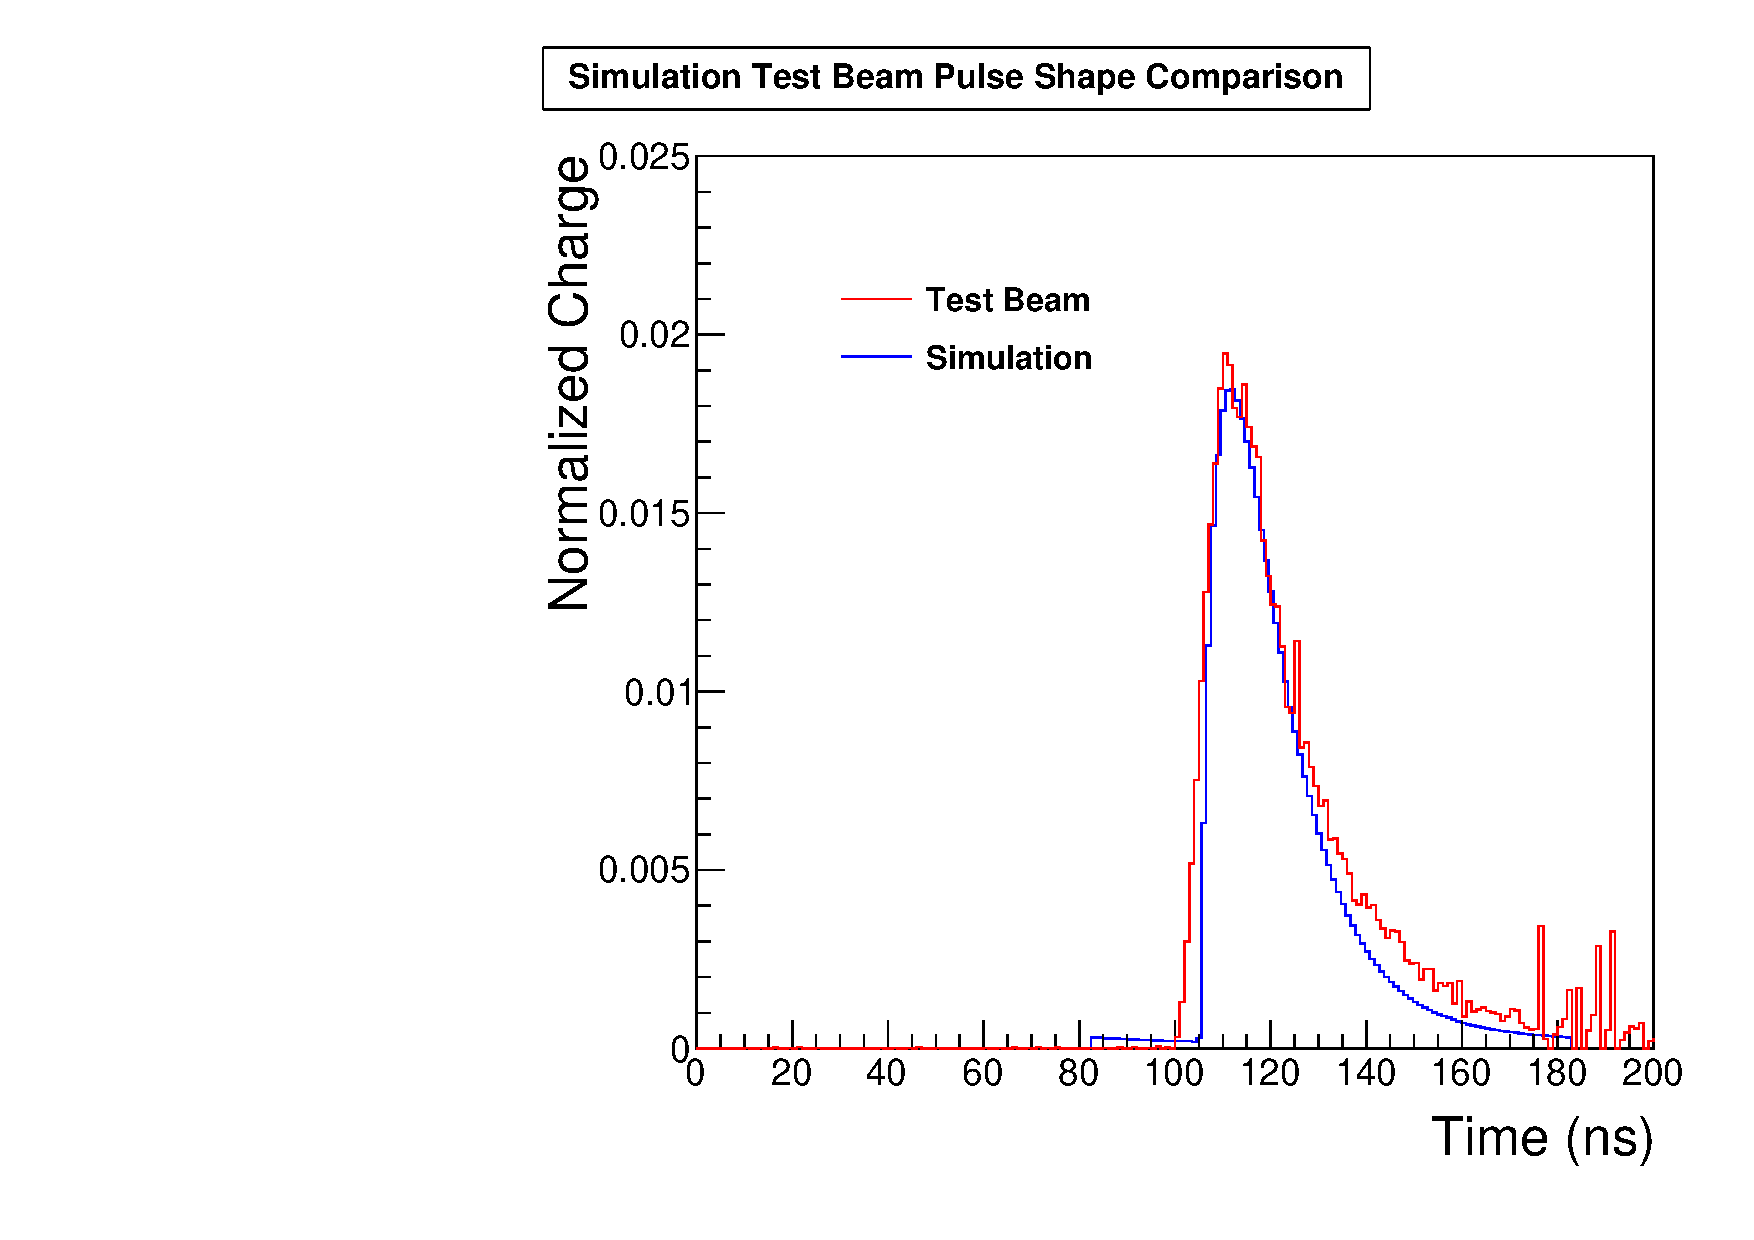
\includegraphics[width=0.495\linewidth]{Figures/125Comparison.pdf}
\caption{Histogram of the pulse shapes from the simulation and the test beam overlapping for comparison purposes. On the left the charge range is 10,000-29,000 fC on the right is 125,000-168,000 fC}
\label{fig:3comparison_together}
\end{figure}

\section{Conclusions}

The creation of the simulation was a very helpful tool in understanding the details of how a SiPM works. It is also a very useful illustration for how it work and it can be easily adjust for future modifications. Some of the plots used in this paper to explain how a SiPM works were created using this simulation. The analysis of the simulation, however, shows that there is still some major flaws with the simulation. The pulse shape comparison shows that the simulation shape is significantly narrower in the base than the actual pulse shape. In addition, the non-linearity in the simulation is much smaller than measurements made using an actual SiPM. The reasons for these discrepancies are still being investigated, but there are several leads. Among them are the changing recharge times and other affects such as the scintillator tiles and QIE chips not yet taken into account in the simulation. 

\end{document}
